\chapter{Simulation} \label{chap:simulation}
\section{Implementation}
A simulation toolbox was implemented in Matlab to model scanning laser range-finder measurements and test observer schemes. The main components of the simulation are:
\begin{itemize} \setlength\itemsep{-2mm}
\item rigid body trajectory computation;
\item solid object modelling;
\item range measurement simulation;
\item noise modelling;
\item observer implementation.
\end{itemize}

\IncMargin{2em}	
	\begin{algorithm}
	\DontPrintSemicolon
	\SetKwFunction{loadsettings}{loadsettings}
	\SetKwFunction{initialisesensor}{initialisesensor}
	\SetKwFunction{initialiseenvironment}{initialiseenvironment}
	\SetKwFunction{initialiseobserver}{initialiseobserver}
	\SetKwFunction{computerange}{computerange}
	\SetKwFunction{addnoise}{addnoise}
	\SetKwFunction{estimatestate}{estimatestate}
	\SetKwFunction{updatestate}{updatestate}
	\SetKwFunction{identifyobject}{identifyobject}	
	\KwData{\\
	%CHANGE THESE TO LETTERS
	$n_{steps}$ - no. steps in simulation\\
	$\mathbf{X}_s$ - sensor pose and scan direction\\
	$\mathbf{X}_e$ - cube and background pose, points and triangles\\
	$\hat{\mathbf{X}}_c$ - estimate of the pose and size of the cube\\
	$c$ - (\texttt{true}/\texttt{false}) current range measurement is of cube or not\\
	$\mathbf{r}$ - ground truth range\\
	$\tilde{\mathbf{r}}$ - measured range\\
	$\hat{\mathbf{r}}$ - predicted range from state estimate\\
	$\bm{\alpha}$ - angle of incidence for each range measurement\\
	$\mathbf{m}$ - index of triangle measured\\
	$\bm{\theta}$ - scan angle in sensor frame\\
	$\bm{\Theta}$ - set of scan angles that return range measurement\\
	}
	\Begin{
		$settings \leftarrow $\loadsettings\\
		$\mathbf{X}_s \leftarrow \initialisesensor(settings)$\\
		$\mathbf{X}_e  \leftarrow \initialiseenvironment(settings)$\\
		\initialiseobserver\\
		\For{$ii \leftarrow 1$ \KwTo $n_{steps}$}{ \label{rangesloop}
			\If{$\bm{\theta}[ii] \in \bm{\Theta}$}{ \label{FOV}
				$[\mathbf{r}[ii],\bm{\alpha}[ii],\mathbf{m}[ii]] \leftarrow \computerange(\mathbf{X}_s[ii],\mathbf{X}_e[ii])$
			}
		}
		$\tilde{\mathbf{r}} = \addnoise(\mathbf{r},\bm{\alpha},\mathbf{m},settings)$ \label{addnoise}\\
		\For{$ii \leftarrow 1$ \KwTo $n_{steps}$}{ \label{observerloop}
			$\hat{\mathbf{X}}_c[ii+1] \leftarrow \estimatestate(\hat{\mathbf{X}}_c[ii])$\\
			\If{$\bm{\theta}[ii] \in \bm{\Theta}$}{
				$\hat{\mathbf{r}}[ii] \leftarrow \computerange(\mathbf{X}_s[ii],\hat{\mathbf{X}}_c[ii])$\\
				$c \leftarrow \identifyobject(c,\tilde{\mathbf{r}})$ \label{object}\\
				\If{$c$}{
					$\hat{\mathbf{X}}_c[ii+1] \leftarrow \updatestate(\hat{\mathbf{X}}_c[ii+1],\mathbf{X}_s[ii],\hat{\mathbf{r}},\tilde{\mathbf{r}})$
				}
			}
		}
	}
	\caption{Scanning range-finder and state observer simulation} \label{main}
	\end{algorithm}
	
The notation employed here and throughout the rest of the report uses the following conventions:
\begin{itemize} \setlength\itemsep{-2mm}
\item \textit{plain text} variables: single values;
\item \textit{bold lowercase} variables: vectors;
\item \textit{bold uppercase} variables: matrices
\item An array formed by replicating a variable $\mathbf{a}$ in an $n \times m$ block array is denoted $\mathbf{a}_{n \times m}$.
\item In many cases, a variable such as the sensor position $\mathbf{p}_s(t)$ represents a set of elements, each corresponding to the value at a certain time $t$. These will be referred to by the form of the value at a single time. For example, a matrix where each column represents a different position vector is used to represent $\mathbf{p}_s(t)$, but it will be described as a vector as this is the form of a single position.
\end{itemize}

A high level description of the simulation is provided in Algorithm \ref{main}.
First, a settings file is loaded. The most important settings determined here are the trajectories of the sensor and environment objects, the scanning behaviour of the sensor and the observer update function.
Next, the sensor class instance is initialised with \texttt{initialisesensor}. This requires computation of the pose and scanning directions of the sensor over time. Similarly, initialisation of the environment through \texttt{initialiseenvironment} requires computation of the pose of each rigid body comprising it. The surfaces of the bodies are then represented with a set of points and corresponding triangles. The position of each point with respect to the inertial frame $\{F\}$ is computed at each time step. The settings file provides the initial conditions with which the observer is initialised in \texttt{initialiseobserver}. 
Beginning on line \ref{rangesloop}, the state of the sensor and environment are used to compute the ground truth range measurements $\mathbf{r}$ at each time step. The incidence angle between the scan direction and object, as well as the index of the triangle hit are also stored as they will be required for sensor noise modelling. This is performed with a parallel \texttt{for} loop to speed up computation. Line \ref{FOV} ensures ranges are only computed when the current scan direction is within the sensor's field of view.
In line \ref{addnoise}, noise is simulated and added to the ground truth ranges to produce the measured ranges $\tilde{\mathbf{r}}$.
The \texttt{for} loop beginning on line \ref{observerloop} begins the observer simulation. 
At each time step, \texttt{estimatestate} estimates the state of the cube $\hat{\mathbf{X}}_c$ from the previous state with the kinematics model in \ref{kinematics}.
From the sensor state $\mathbf{X}_s$ and the estimated state of the cube $\hat{\mathbf{X}}_c$, \texttt{computerange} is used to determined the predicted range measurement $\hat{\mathbf{r}}$.
The variable $c$ indicates whether the current range measurement corresponds to the cube or the background. On line \ref{object} the measured ranges and previous value of $c$ are used to determine whether the current measurement corresponds to the cube. If it does, the cube state estimate $\hat{\mathbf{X}}_c$ is updated using the previous state estimate, current sensor state, and the predicted and measured ranges.


\subsection{Rigid Body Motion} \label{motion}
To simulate range measurements the pose of the sensor and the objects comprising the environment must be computed at each time step. The computations required to do so can be reduced by taking into account the kinds of motion that must be simulated. This section details how the pose of the sensor and objects is represented and computed, which is used in the functions \texttt{initialisesensor}, \texttt{initialiseenvironment} and \texttt{estimatestate} referenced in Algorithm \ref{main}.

The observer actually computes the \textit{relative} position between the sensor and cube and simply uses knowledge of the sensor pose to determine the pose of the cube in the inertial frame. There is no need to simulate complex sensor motions because the motion of the cube can be adjusted to achieve the same result. The only requirement of the sensor motion is that measurements of a large range of the environment are acquired to ensure that the entire target object can be viewed. The scanning behaviour of the sensor is to rotate back and forth about the $z$-axis of the body fixed frame $\{A\}$. To provide a rectangular field of view, the motion of the sensor is therefore limited to constant velocity rotation about $y$-axis of inertial frame $\{F\}$.

The environment is modelled with two rigid bodies: a cube to be observed as the target object, and a stationary rectangular prism enclosing the sensor and cube acting as the background. The various cube motions that will be simulated to test the observer's performance can be classed in terms of the wrench matrix of the cube as either
\begin{enumerate}
\item ${\textbf{W}_c} = \textbf{0}$
\item ${\textbf{W}_c} \neq \textbf{0}$
\end{enumerate}

For case 1. the wrench and screw are constant so only the initial value is required. It is more efficient to represent the pose of a rigid body with just position and orientation in this case. The pose can be quickly computed by interpolating between an initial and final pose. For case 2. the screw, twist and wrench must be integrated numerically.

\subsubsection{Interpolation}
For the case of zero wrench, the pose of the body can be represented with a position vector $\mathbf{p}_i$ and an orientation quaternion $\mathbf{q}_i$. A trajectory of $k$ poses at times 
$\mathbf{t} =
\begin{bmatrix}
	t_1 & t_2 & t_3 & \dots & t_k
\end{bmatrix}$,
is computed by interpolating from an initial pose $\{\mathbf{p}_0,\mathbf{q}_0\}$ to a final pose $\{\mathbf{p}_k,\mathbf{q}_k\}$.

The array of position vectors
$\mathbf{P}= \begin{bmatrix}
\mathbf{p}_1 & \mathbf{p}_2 & \mathbf{p}_3 & \dots & \mathbf{p}_k
\end{bmatrix}$
 are computed with:
\begin{equation}
	\mathbf{P} = 
	(\mathbf{1}_{3 \times k}){\mathbf{p}_1} + (\mathbf{p}_k - \mathbf{p}_1)\frac{\mathbf{t}-{t_1}(\mathbf{1}_{1 \times k})}{t_k - t_1}
\end{equation}

Spherical linear interpolation is used to compute the array of orientation quaternions
$\mathbf{Q}= \begin{bmatrix}
	\mathbf{q}_1 & \mathbf{q}_2 & \mathbf{q}_3 & \dots & \mathbf{q}_k
\end{bmatrix}$
at each time step:
\begin{equation} \label{slerp}
	\mathbf{Q} = \frac{\mathbf{q}_1\sin((\mathbf{1}_{[1 \times k]}-\mathbf{t})\theta) + \mathbf{q}_k\sin(\mathbf{t}\theta)}{\sin(\theta)}
\end{equation}
where
\begin{equation}
	\theta = \cos^{-1}(\mathbf{q}_1 \cdot \mathbf{q}_k)
\end{equation}

This interpolation method is used to compute the trajectory of the sensor. To acquire multiple views of the  entire cube, the sensor must pan back and forth several times. This is achieved by first reversing the trajectory and concatenating with the original to produce the looped trajectories $\mathbf{P}_{loop}$ and $\mathbf{Q}_{loop}$:
\begin{equation}
	\mathbf{P}_{loop}= 
	\begin{bmatrix}
		\mathbf{p}_1 & \mathbf{p}_2 & \mathbf{p}_3 & \dots & \mathbf{p}_k &
		\mathbf{p}_{k} & \mathbf{p}_{k-1} & \mathbf{p}_{k-2} & \dots & \mathbf{p}_1
	\end{bmatrix}
\end{equation}
\begin{equation}
	\mathbf{Q}_{loop}= 
	\begin{bmatrix}
		\mathbf{q}_1 & \mathbf{q}_2 & \mathbf{q}_3 & \dots & \mathbf{q}_k &
		\mathbf{q}_{k} & \mathbf{q}_{k-1} & \mathbf{q}_{k-2} & \dots & \mathbf{q}_1
	\end{bmatrix}
\end{equation}

This looped trajectory is repeated $k$ times to produce multiple back and forth scans:
\begin{equation}
	\mathbf{P} = ({\mathbf{P}_{loop}})_{1 \times k}
\end{equation}
\begin{equation}
	\mathbf{Q} = ({\mathbf{Q}_{loop}})_{1 \times k}
\end{equation}


\subsubsection{Numerical Integration} \label{integration}
The time evolution of the screw, twist and wrench is computed iteratively from initial conditions by numerically integrating the ODEs in section \ref{kinematics}. For a rigid body with an associated reference frame $\{X\}$, moving with constant acceleration:

\begin{equation}
	\mathbf{S}_X(t+\delta t) = \mathbf{S}_X(t)\exp({\delta t {\mathbf{T}_X(t)}})
\end{equation}

\begin{equation}
	\mathbf{T}_X(t+\delta t) = \mathbf{T}_X(t) + \delta t \mathbf{W}_X(t)
\end{equation}

\begin{equation}
	\mathbf{W}_X(t+\delta t) =\mathbf{W}_X(t)
\end{equation}

Though a higher order integration method, such as Runge-Kutta could be used to compute a trajectory that more accurately represents a constant acceleration, this is not strictly necessary. The observer performance is unlikely to be affected by how constant the acceleration is. Furthermore, it is likely that the experimentally collected data will have even larger variations in acceleration.

To simplify the code, the position vector and orientation quaternion are computed from the screw matrix. This allows the same functions to be used in either the interpolation or numerical integration cases. Multiplying the points that make up the rigid objects can also be done more compactly with quaternions.

\subsection{Sensor modelling: \texttt{initialisesensor}}
The motion model below is used to compute the pose of the sensor. The scanning model is used to compute the set of scanning directions. These actions are performed in the $\texttt{initialisesensor}$ function in Algorithm \ref{main}
\subsubsection{Motion}
The state of the sensor $\mathbf{X}_{s}(t)$ consists of terms corresponding to its motion and scanning operation. Since the motion of the sensor is restricted to zero acceleration, the state of sensor can be computed with the interpolation method and represented with position, orientation and scanning direction. 
\begin{equation}
	\mathbf{X}_{s}(t) = \{\mathbf{p}_s(t),\mathbf{q}_s(t),{^{A}\mathbf{d}(t)}\}
\end{equation}

Since it has a stationary position, the position of the sensor over time is fixed at the origin of the inertial frame $\{F\}$.
\begin{equation}
	\mathbf{p}_1 = \mathbf{p}_2 = \mathbf{p}_3 = \dots =  \mathbf{p}_k = 
	\begin{bmatrix}
		0 \\ 0 \\ 0
   	\end{bmatrix}
\end{equation}
										
The sensor rotates between $-\phi$ and $\phi$ about the $y$-axis of inertial frame $\{F\}$. Thus, its orientation is computed by interpolating between $\mathbf{q}_1$ and $\mathbf{q}_k$ with equation \ref{slerp}.
	
\begin{equation}
	\mathbf{q}_1 = \begin{bmatrix}
				 	\cos(-\phi/2) \\
				 	\sin(-\phi/2){\begin{bmatrix}
								 	0 \\ 1 \\ 0
							   	 \end{bmatrix}}
				 \end{bmatrix}
				 = \begin{bmatrix}
		 		   		\cos(\phi/2) \\ 0 \\ -\sin(\phi/2) \\ 0
				   \end{bmatrix}
\end{equation}

\begin{equation}
	\mathbf{q}_k = \begin{bmatrix}
				 	\cos(\phi/2) \\
				 	\sin(\phi/2){\begin{bmatrix}
								 	0 \\ 1 \\ 0
							   	 \end{bmatrix}}
				 \end{bmatrix}
				 = \begin{bmatrix}
		 		   		\cos(\phi/2) \\ 0 \\ \sin(\phi/2) \\ 0
				   \end{bmatrix}
\end{equation}

\subsubsection{Scanning} \label{sec:scanmodel}
The scanning behaviour of the sensor depends on the particular model used. The \textit{Hokuyo UBG 04-LX} scanning laser range-finder will be modelled as it was the sensor used to conduct experiments in this project. This sensor produces a 785nm laser beam, projected at a precise direction. It measures the characteristics of the reflected beam to determine the position to the nearest object in the direction of the beam. The direction of the laser beam is varied by reflecting it off a rotating mirror. The rotation means that the beam direction effectively rotates with a constant velocity in a single plane. A portion of the field of view of the laser beam is obscured, so measurements will not be returned in a certain region of each revolution.

The vector ${^{A}\mathbf{d}(t)}$ will be used to model this scanning behaviour.
To accurately model this, the following parameters are used:
\begin{itemize}
\item field of view $\mathbf{\Theta}$: The vector ${^{A}\mathbf{d}(t)}$ rotates anti-clockwise about the $z$ axis of the sensor frame $\{A\}$. Measurements are only taken when the scan angle about is between $-\theta$ and $\theta$ about the $-z$-axis of the sensor frame $\{A\}$. In practice, the field of view is implemented as the start angle $-\theta$, direction of rotation and angular range $2\theta$.
\item number of scans $n_{scans}$: This represents the number of scan angles in a single revolution. Since measurements are limited by the field of view of the sensor, the actual number of measurements per second is $n_{ranges} = \frac{2\theta}{2\pi}n_{scans}$. The angular resolution is $d\theta = \dfrac{2\pi}{n_{scans}}$.
\item revolutions per second $\Omega$: This is measured in Hz and gives the length of each time step $d\tau = \dfrac{1}{n_{scans}\Omega}$
\item $n_{loops}$: The number of back and forth repeats of the sensor trajectory.
\end{itemize}
From these parameters the scanning direction ${^{A}\mathbf{d}(t)}$ is created. At each time $t$, ${^{A}\mathbf{d}(t)}$ is either a unit vector indicating the direction of measurement in the sensor frame, or has $\mathbf{0}$ magnitude, corresponding to when ${^{A}\mathbf{d}(t)}$ is outside the field of view and the sensor is not returning a measurement.

\begin{equation}
^{A}\mathbf{d}(t) =
	\begin{cases} 
	      \hfill \begin{bmatrix}
	      		\cos(-\theta + 2\pi t') \\
	      		-\sin(-\theta + 2\pi t') \\
	      		0
	      	\end{bmatrix}    \hfill & \text{ if $t' \leq \theta/\pi$, $t' = k\delta\tau$  $\forall k \in \mathbb{N}$} \\
	      \hfill \mathbf{0}_{3 \times 1} \hfill & \text{ if $t' > \theta/\pi$, $t' \neq k\delta\tau$  $\forall k \in \mathbb{N}$} \\
	\end{cases} 
\end{equation}
where
\begin{equation}
t' = \mod(t,1/d\theta)\:d\theta
\end{equation}

Figure \ref{fig:scanningparameters} shows the frame $\{A\}$ fixed to the sensor and the scan direction ${^{A}\mathbf{d}(t)}$. At time $t' = 0$, the first scan direction ${^{A}\mathbf{d}_0}$ has an angular displacement of $-\theta$ about the $z$-axis from the forward facing $x$-direction. After each time step $d\tau$, the scan direction rotates by $d\theta$ about the $z$-axis. There are $n_{ranges}$ scan directions within the field of view of the sensor. The entire revolution is divided into $n_{scans}$ scan directions.
\begin{figure}
	\centering
	\tdplotsetmaincoords{60}{-130}
	%\tdplotsetmaincoords{0}{0}
	\begin{tikzpicture} [scale = 2,tdplot_main_coords] %fix main coords!!!

		%field of view
		\path [fill={rgb:black,1;white,3}] (2,1,0) arc (45:135:2.828) -- (0,0,0) -- (2,1,0);
		\draw [dashed,->](0, 0, 0)--(-4, 2, 0);
		\draw [dashed,->](0, 0, 0)--(4, 2, 0);
		\draw [dashed,->](0, 0, 0)--(-3.8, 2.358, 0);
		\draw [dashed,->](0, 0, 0)--(-3, 3.317, 0);
		\draw [dashed,->](0, 0, 0)--(-4.18, 1.589, 0);
		\draw [dashed,->](0, 0, 0)--(4.18, 1.589, 0);
		\draw[dashed] (2,1,0) arc (45:135:2.828);
		\draw[<->] (0.5,0.25,0) arc (45:90:0.707);
		\draw[<->] (-0.5,0.25,0) arc (135:90:0.707);
		\draw[<->] (-3.2,1.21,0) arc (165:145:1);
		\draw[<->] (-3.05,1.53,0) arc (145:126:1);
		\draw[<->] (3.2,1.21,0) arc (15:35:1);
		
		%Frame {A}
		\draw [thick,->](0, 0, 0)--(-3, 0, 0) node[anchor=west]{$y$};
		\draw [thick,->](0, 0, 0)--(0, 3, 0) node[anchor=north east]{$x$};
		\draw [thick,->](0, 0, 0)--(0, 0, 1.5) node[anchor=south]{$z$};
		
		%labels
		\node [black,anchor=north west] at (0.5,0.5,0) {$\theta$};
		\node [black,anchor=north] at (-0.05,0.5,0) {$\theta$};
		\node [black,anchor=south east] at (-3.2,1.21,0) {$d\theta$};
		\node [black,anchor=south east] at (-3.05,1.53,0) {$d\theta$};
		\node [black,anchor=east] at (3.2,1.21,0) {$d\theta$};
		\node [black,anchor=west] at (0.1,-0.2,0) {$\{A\}$}; 
		\node [black,anchor=west] at (-4.18, 1.59, 0) {$^{A}\mathbf{d}_{n_{scans}}$}; 
		\node [black,anchor=north] at (-4.05,1.95,0) {$^{A}\mathbf{d}_{0}$}; 
		\node [black,anchor=north] at (-3.8, 2.358, 0) {$^{A}\mathbf{d}_{1}$}; 
		\node [black] at (-3.7, 3.1, 0) {$\bm{\cdots}$}; 
		\node [black,anchor=north] at (-3, 3.317, 0) {$^{A}\mathbf{d}_{k}$}; 
		\node [black,anchor=east] at (4,2,0) {$^{A}\mathbf{d}_{n_{ranges}}$};
		\node [black,anchor=south east] at (4.18, 1.59, 0) {$^{A}\mathbf{d}_{n_{ranges}+1}$}; 
		
	\end{tikzpicture}
	  \caption{Scanning parameters}
	  \label{fig:scanningparameters}
\end{figure}





To simulate range measurements, the scan direction is required in the inertial frame $\{F\}$. This is computed by multiplying with the screw matrix of the sensor.
\begin{equation}
	\begin{array}{lcl}
	{^{F}\mathbf{d'}(t)} & = & \mathbf{S}_s(t)\:{^{A}\mathbf{d'}(t)} \\
	& = & {^{F}_{F}\mathbf{S}^{}_{A}(t)}\:{^{A}\mathbf{d'}(t)}
	\end{array}
\end{equation}

\subsection{Environment Modelling: \texttt{initialiseenvironment}}
Object + background make up infinite dimensional system. State of cube to be estimated is finite-dimensional.
Environment should be infinite dimensional - will only model a single background object.
still taking measurements of an infinite dimensional system- though represented discretely for computational load. Does not make a difference to observer. Observer doesn't know background is a single rigid body. Could be anything.

\subsubsection{Motion}
The pose of each object represents the pose of its centre of mass. As described in section \ref{motion} the pose is computed with interpolation for the case of zero wrench, and numerical integration in the case of non-zero wrench. The pose of the objects making up the environment is computed with the function $\texttt{initialiseenvironment}$ in Algorithm \ref{main}. This function also creates the points and triangles that model the surface of the objects which is described below.

\subsubsection{Rigid Objects}
The environment is represented with two rectangular prisms; the cube and a larger rectangular prism enclosing both the sensor and cube, to represent the background. These objects are modelled as an ordered set of 8 points in the inertial reference frame and an ordered set of 12 triangles formed by these points. Each triangle is represented by a set of 3 integers, indicating the index of the three points that make up its vertices.

The cube points in body frame $\{B\}$ are represented with the matrix ${^{B}\mathbf{P}}$.
\begin{equation}
	{^{B}\mathbf{P}} = \frac{1}{2}s
	\begin{bmatrix*}[r]
		-1  &  -1  &  -1  &  -1  &   1  &   1  &   1  &  \hspace{0.75em} 1 \\
		-1  &  -1  &   1  &   1  &  -1  &  -1  &   1  &  1 \\
		-1  &   1  &  -1  &   1  &  -1  &   1  &  -1  &  1 
	\end{bmatrix*}
\end{equation}
To represent these points in the inertial frame $\{F\}$, ${^{F}\mathbf{P}}$ is computed by rotating each point with the orientation quaternion of frame $\{B\}$ using equation \ref{quatrot} before adding the vector representing the translation of $\{B\}$ from $\{F\}$.

The triangles are represented with the matrix $\mathbf{T}$. Each triangle is represented by a row. The elements of these rows are the three vertices of the triangle and the index corresponds a point in ${^{F}\mathbf{P}}$.
\begin{equation}
	\mathbf{T} = 
	\begin{bmatrix}
	1 & 2 & 3 \\
	2 & 4 & 3 \\
    4 & 3 & 7 \\
    4 & 8 & 7 \\
    5 & 6 & 7 \\
    8 & 6 & 7 \\
    2 & 6 & 5 \\
    2 & 1 & 5 \\
    2 & 6 & 8 \\
    2 & 4 & 8 \\
    1 & 5 & 7 \\
    1 & 3 & 7
	\end{bmatrix}
\end{equation}

The points and triangles are shown in Figure \ref{fig:triangles}.
\begin{figure}
\centering
\tdplotsetmaincoords{60}{10}
	\begin{tikzpicture} [scale = 2,tdplot_main_coords] %fix main coords!!!

		%Frame {B}
		\draw [thick,->](0, 0, 0)--(-2.5, 0, 0) node[anchor=east]{$y$};
		\draw [thick,->](0, 0, 0)--(0, 3.5, 0) node[anchor=east]{$x$};
		\draw [thick,->](0, 0, 0)--(0, 0, 2.5) node[anchor=south]{$z$};
		\node at (0.1,-0.25,0) {\{B\}};
		%points		
		\node[anchor=west] at ( 1,-1,-1) {$1$};
		\node[anchor=west] at ( 1,-1, 1) {$2$};
		\node[anchor=east] at (-1,-1,-1) {$3$};
		\node[anchor=east] at (-1,-1, 1) {$4$};
		\node[anchor=west] at ( 1, 1,-1) {$5$};
		\node[anchor=west] at ( 1, 1, 1) {$6$};
		\node[anchor=east] at (-1, 1,-1) {$7$};
		\node[anchor=east] at (-1, 1, 1) {$8$};

		\node[draw,circle,inner sep=1.5pt,fill] at ( 1,-1,-1) {};
		\node[draw,circle,inner sep=1.5pt,fill] at ( 1,-1, 1) {};
		\node[draw,circle,inner sep=1.5pt,fill] at (-1,-1,-1) {};
		\node[draw,circle,inner sep=1.5pt,fill] at (-1,-1, 1) {};
		\node[draw,circle,inner sep=1.5pt,fill] at ( 1, 1,-1) {};
		\node[draw,circle,inner sep=1.5pt,fill] at ( 1, 1, 1) {};
		\node[draw,circle,inner sep=1.5pt,fill] at (-1, 1,-1) {};
		\node[draw,circle,inner sep=1.5pt,fill] at (-1, 1, 1) {};	
		
		%cube lines
		\draw (-1,-1,-1)--(-1,-1, 1);   %1-2
		\draw (-1,-1,-1)--(-1, 1,-1);   %1-3
		\draw (-1,-1,-1)--( 1,-1,-1);   %1-5
		\draw (-1,-1, 1)--(-1, 1, 1);   %2-4
		\draw (-1,-1, 1)--( 1,-1, 1);   %2-6	
		\draw (-1, 1,-1)--(-1, 1, 1);   %3-4 	 
		\draw (-1, 1,-1)--( 1, 1,-1);   %3-7	
		\draw (-1, 1, 1)--( 1, 1, 1);   %4-8 
		\draw ( 1,-1,-1)--( 1,-1, 1);   %5-6	
		\draw ( 1,-1,-1)--( 1, 1,-1);   %5-7 
		\draw ( 1,-1, 1)--( 1, 1, 1);   %6-8 
		\draw ( 1, 1,-1)--( 1, 1, 1);   %7-8 
		%triangle lines
		\draw [dashed] ( 1,-1, 1)--(-1,-1,-1);   %2-3
		\draw [dashed] (-1,-1, 1)--(-1, 1,-1);   %4-7
		\draw [dashed] ( 1, 1, 1)--(-1, 1,-1);   %6-7 
		\draw [dashed] ( 1,-1, 1)--( 1, 1,-1);   %2-5
		\draw [dashed] ( 1,-1, 1)--(-1, 1, 1);   %2-8
		\draw [dashed] ( 1,-1,-1)--(-1, 1,-1);   %1-7
		
	\end{tikzpicture}
	  \caption{Cube modelled with an ordered set of points and corresponding triangles}
	  \label{fig:triangles}
\end{figure}





\subsection{Measurement Modelling}
	\subsubsection{Range Computation: \texttt{computerange}}
	This section describes the implementation used in the $\texttt{computerange}$ function in Algorithm \ref{main}.
	
	Given the screw matrix (in the inertial frame) and scan direction (in the body fixed frame) of the sensor, the position and scan direction in the inertial frame are determined.
	The distance to the nearest environment object from this point, along the scan direction is determined with the M{\"o}ller-Trumbore ray-triangle intersection algorithm, shown in Algorithm \ref{intersectionalgorithm}.
	
	Figure \ref{fig:raytriangle} shows a simplified scenario involving the intersection of a ray with a single triangle. In practice, the algorithm is vectorised to compute the intersections with a \textit{set} of triangles. In this vectorised implementation, many variables represent a matrix whose columns are each vectors. These variables will still be described as vectors to emphasise the operation of the M{\"o}ller-Trumbore algorithm, rather than the specific implementation details.	\begin{figure}
	\tdplotsetmaincoords{60}{-20}
	\begin{tikzpicture} [scale = 2,tdplot_main_coords] %fix main coords!!!
		
		%triangle
		\node[draw,circle,inner sep=1.5pt,fill] at ( 1,6,-1) {};
		\node[draw,circle,inner sep=1.5pt,fill] at ( 0,6, 1) {};
		\node[draw,circle,inner sep=1.5pt,fill] at (-2,6,-1) {};
		\node [black,anchor=east] at (-2,6,-1) {$\mathbf{v}_1$};
		\node [black,anchor=west] at ( 1,6,-1) {$\mathbf{v}_2$}; 
		\node [black,anchor=south] at ( 0,6, 1) {$\mathbf{v}_3$}; 
		\draw ( 1,6,-1)--( 0,6, 1); 
		\draw ( 1,6,-1)--(-2,6,-1);
		\draw ( 0,6, 1)--(-2,6,-1);
		\node [black,anchor=east] at (-0.5,6,-1) {$\mathbf{e}_1$};
		\node [black,anchor=west] at ( -1,6,0.5) {$\mathbf{e}_2$}; 
		%ray
		\draw [dashed,->](0, 0, 0)--(-0.5, 8, 0);
		\draw [thick,->](0, 0, 0)--(-0.5/5, 8/5, 0);
		%computation stuff
		
		%Frame {A}
		\draw [thick,->](0, 0, 0)--(-1, 0, 0) node[anchor=east]{$y$};
		\draw [thick,->](0, 0, 0)--(0, 1, 0) node[anchor=south west]{$x$};
		\draw [thick,->](0, 0, 0)--(0, 0, 1) node[anchor=south]{$z$};
		\node [black,anchor=west] at (0,0,0) {$\{A\}$}; 
		
	\end{tikzpicture}
	  \caption{Ray-triangle intersection}
	  \label{fig:raytriangle}
\end{figure}




	
	The output variables are first initialised to the case that there is no intersection with the scanning direction. $x$ is set to \texttt{false} and the range, angle and triangle index outputs are set to return \texttt{NaN}.
	
	On line \ref{line: vertex}, the set of points $\mathbf{P}$ are indexed using the columns of the triangle matrix $\mathbf{T}$ to extract the three vertices corresponding to each triangle.
	The vectors representing the edges sharing vertex $\mathbf{V}_1$ are computed.
	from triangles and points, extract vertices of each triangle.
	The vector $\mathbf{A}$ computed on line \ref{line: origintov1} represents the translation from the ray origin $\mathbf{o}$ to $\mathbf{V}_1$.
	
	The collection of vectors $\mathbf{B}$ is computed on line \ref{line: det} by taking the cross product of the scan direction $\mathbf{d}$ and each edge $\mathbf{E}_2$. The determinant $\bm{\delta}$ of the matrix
	\begin{equation}
		\mathbf{M} = 
			\begin{bmatrix} 
				\mathbf{e}_1 \\
				\mathbf{d}	 \\
				\mathbf{e}_2
			\end{bmatrix}
	\end{equation}
	is computed on line \ref{line: det}. This is first used to determine if the scan direction $\mathbf{d}$ lies in the plane of the triangle by checking if the determinant is close to zero. If so, no intersection can occur. The zero determinant values are then set to \texttt{NaN} to avoid a division by zero later.
	
	Beginning on line \ref{line: alpha}, determinant $\bm{\delta}$ is used to compute the barycentric coordinates $\bm{\alpha}$ and  $\bm{\beta}$, and the distance $\mathbf{s}$ from the origin to the triangle plane along the scan direction $\mathbf{d}$.
	
	The barycentric coordinates are used to determine if the intersection between the scan direction $\mathbf{d}$ and the plane of the triangle lies within the triangle itself. 
	
	The vector $\mathbf{x}$ on line \ref{line: intersectvec} now indicates which triangles intersected with the scan direction. $\mathbf{x}$ is used to mask the ranges to the triangles $\mathbf{s}$, to give $\mathbf{r}$; the range to each intersecting triangle. 
	
	The minimum range $r$ and triangle index $m$ are determined before computing the angle of incidence $\theta$ between $\mathbf{d}$ and the closest triangle.
	
	\begin{singlespace}
	\IncMargin{2em}
	\begin{algorithm}
	\DontPrintSemicolon
	\SetKwInOut{Input}{input}\SetKwInOut{Output}{output}
	\SetKwFunction{size}{size}
	\SetKwFunction{any}{any}
	\SetKwFunction{min}{min}
	\SetKwFunction{find}{find}
	
	\Input{$\mathbf{o}$ - ray origin\\
		   $\mathbf{d}$ - ray direction vector\\
		   $\mathbf{P}$ - cube in inertial frame \\
		   $\mathbf{T}$ - triangle matrix}
	\Output{$x$ - True/False - measurement corresponds to object\\
			$r$ - distance to object in m\\
			$\theta$ - incidence angle in rad\\
			$m$ - index of triangle hit}
	\Begin{
		\tcc{initialise outputs}
		$x \longleftarrow 0$\\
		$r \longleftarrow NaN$\\
		$\theta \longleftarrow NaN$\\
		$m \longleftarrow NaN$\\
		\tcc{triangle vertexes and edges}
		$\mathbf{V}_1 \longleftarrow \mathbf{P}[\mathbf{T}[:,1]]$ \label{line: vertex}\\
		$\mathbf{V}_2 \longleftarrow \mathbf{P}[\mathbf{T}[:,2]]$\\
		$\mathbf{V}_3 \longleftarrow \mathbf{P}[\mathbf{T}[:,3]]$\\
		$\mathbf{E}_1 \longleftarrow \mathbf{V}_2 - \mathbf{V}_1$\\
		$\mathbf{E}_2 \longleftarrow \mathbf{V}_3 - \mathbf{V}_1$\\
		$m = \size(\mathbf{V}_1,1)$\\
		$\mathbf{A} \longleftarrow \mathbf{o}_{[m \times 1]} - \mathbf{V}_1$ \label{line: origintov1}\\
		\tcc{determinant}
		$\mathbf{B} \longleftarrow \mathbf{d}_{[m \times 1]} \times \mathbf{E}_2$ \label{line: det}\\
		$\bm{\delta} \longleftarrow \mathbf{E}_1 \cdot \mathbf{B}$\\		
		$\mathbf{y} \longleftarrow |\bm{\delta}|\leq\mathbf{0}$\\
		$\bm{\delta}[\mathbf{y}] \longleftarrow \mathbf{NaN}$\\
		\tcc{barycentric coordinates}
		$\bm{\alpha} \longleftarrow (\mathbf{A} \cdot \mathbf{B})/\bm{\delta}$ \label{line: alpha}\\
		$\mathbf{Q} \longleftarrow \mathbf{A} \times \mathbf{E}_1$ *(along dim 2)\\
		$\bm{\beta} \longleftarrow (\mathbf{d}_{[n \times 1]} \cdot \mathbf{Q})/\bm{\delta}$ *(along dim 2)\\
		$\mathbf{s} \longleftarrow (\mathbf{E}_2 \cdot \mathbf{Q})/\bm{\delta}$\\
		\tcc{intersection vector}	
		$\mathbf{z} \longleftarrow \mathbf{y} \textbf{ and } (\bm{\alpha} \geq \mathbf{0}) 
		\textbf{ and } (\bm{\beta} \geq \mathbf{0}) \textbf{ and } (\bm{\alpha}+\bm{\beta} \leq 
		\mathbf{1})$\\
		$\mathbf{x} \longleftarrow \mathbf{z} \textbf{ and } (\mathbf{s} \geq \mathbf{0})$ \label{line: intersectvec} \\
		\If{$\any(\mathbf{x})$}{ 
			$x \longleftarrow 1$\\
			$\mathbf{x}[\textbf{not }\mathbf{x}] \longleftarrow \mathbf{NaN}$\\
			$\mathbf{r} = \mathbf{s} \circ \mathbf{x}$\\
			$r = \min(\mathbf{r})$\\
			$m = \find(\mathbf{r} = r,1)$\\
			$\mathbf{e}_1 \longleftarrow \mathbf{E}_1[t,:]$\\ 
			$\mathbf{e}_2 \longleftarrow \mathbf{E}_2[t,:]$\\ 
			$\mathbf{n} = \mathbf{e}_1 \times \mathbf{e}_2$\\
			$\theta = \texttt{atan2}(|\mathbf{d}\times\mathbf{n}|,\mathbf{d}\cdot\mathbf{n})$\\
			$\theta = \min(\theta,\pi-\theta)$
		}
	}
	\caption{M{\"o}ller-Trumbore ray-triangle intersection} \label{intersectionalgorithm}
	\end{algorithm}
	\end{singlespace}
		
	\subsubsection{Sensor Noise: \texttt{addnoise}}
	In Algorithm \ref{main}, the function \texttt{addnoise} takes the ground truth range measurements and produces the noisy range measurements that the observer will actually receive.
	The noise function $f_s$ is
	\begin{equation}
		\hat{r}(t) = f_s(r(t),\theta(t),\phi(k))
	\end{equation}
	where $\theta(t)$ is the incidence angle of the measurement, $\phi$ represents the surface properties of the object $k$ that was measured.
	
	For the Hokuyo UBG-04LX-F01 sensor used, range measurements taken at various distances and incidence angles were used to estimate the noise model $f_{UBG}$ which is provided in section \ref{sensor_noise}.
	
\subsection{Observer Implementation}
	\textbf{FIGURES ARE USED TO EXPLAIN FUNCTIONS. FIGURES THEMSELVES NEED SOME EXPLAINING - IE TRIANGLES ON SURFACE, NOT INSIDE CUBE FOR ORIENTATION}
	\subsubsection{Estimate: \texttt{estimatestate}}
		The state of the cube at each time step is estimated using the numerical integration method described in section \ref{integration}. This state estimation is implemented in the function \texttt{estimatestate} in Algorithm \ref{main}.
	
	\subsubsection{Object/background sepraration: \texttt{identifyobject}}
		The observer update function will use range measurements to estimate the state of the cube $\mathbf{X}_c$. In order to perform accurately, the observer must only use range measurements that correspond to the cube. The function \texttt{identifyobject} in Algorithm \ref{main} uses range measurements and knowledge of the configuration of the environment to separate measurements of the cube and background.
		
		The binary variable $c$ indicates whether the current range measurement corresponds to cube ($c=\texttt{true}$) or the background ($c=\texttt{false}$). It is assumed that initially the sensor will be observing the background, so $c_0=\texttt{false}$.

		The scheme used to identify range measurements corresponding to the cube is shown in Algorithm \ref{alg:object}. There are two assumptions that may be used.
		\begin{enumerate}
		\item The \textit{difference assumption} relies on the assumption that the cube and background objects are continuous. Differences in consecutive range measurements larger than $\Delta_{max}$ indicate a discontinuity, implying that a new object is being measured. When this occurs, the value of $c$ changes.
		\item The \textit{range assumption} is used when the maximum distance to the cube and minimum distance to the background are restricted. Range measurements within $r_{max}$ correspond to the cube while larger ranges correspond to the background.
		\end{enumerate}
		
		\IncMargin{2em}
		\begin{algorithm}
		\DontPrintSemicolon
		\SetKwInOut{Input}{input}\SetKwInOut{Output}{output}
	
		\Input{ $differenceAssumption$ - true/false\\
			   $rangeAssumption$ - true/false\\
			   $\Delta_{max}$ - max diff between measurements of same object\\
			   $r_{max}$ - max range for cube\\
			   $c$ - true/false - current measurement is of cube\\
			   $\mathbf{r}_{i+1}$ - distance to object at $t = i+1$\\
			   $\mathbf{r}_{i}$ - distance to object at $t = i$}
		\Output{$c$ - true/false}
		\Begin{				
			\If{$differenceAssumption$}{
				\If{$|\mathbf{r}_{i+1}-\mathbf{r}_{i}| > \Delta_{max}$}{
					$c = \mod(c + 1,2)$
				}
			}
			\If{$rangeAssumption$}{
				\If{$\mathbf{r}_{i+1} > r_{max}$}{
					$c = 0$
				}
			}
		}
		\caption{Target/background object separation} \label{alg:object}
		\end{algorithm}
		
	\subsubsection{Update: \texttt{updatestate}} 
		If the \texttt{identifyobject} function identifies a range measurement as corresponding to the cube, the \texttt{updatestate} function is used to update the state estimate of the cube $\hat{\mathbf{X}}_c$. $\hat{\mathbf{X}}_c$ is updated using the previous cube state estimate, current sensor state, and sets of measured and predicted range measurements chosen according to a set of indexes $\mathbf{a}(t)$. 
		\begin{equation}
			\hat{\mathbf{X}}_{c}(k+1) = f(\mathbf{X}_{s}(t),\hat{\mathbf{X}}_{c}(k),\mathbf{r}(\mathbf{a}(t)),\hat{\mathbf{r}}(\mathbf{a}(t)))
		\end{equation}	
		The pose of $\hat{\mathbf{X}}_c$ is corrected by adjusting $\hat{\mathbf{S}}_c$, $\hat{\mathbf{T}}_c$ or $\hat{\mathbf{W}}_c$, or some combination of the three.
		The orientation is adjusted by rotating  about an axis $\mathbf{r}_{update}$. The position is adjusted by translating in the direction of $\mathbf{p}_{update}$
		$\mathbf{r}_{update}$ and $\mathbf{p}_{update}$ are scaled differently, depending on whether they are applied to $\hat{\mathbf{S}}_c$, $\hat{\mathbf{T}}_c$ or $\hat{\mathbf{W}}_c$.
		The size update $s_{update}$ is independent of the pose update scheme used.
		
		\textbf{Input ranges:}\\
			A set of four range measurements forming a quadrilateral are used in the state update. The four ranges are chosen with an ordered sequence of indexes $u(t)$. At a time step $ii$, the set of time steps used is in the update function is
			\begin{equation}
				\mathbf{u}(ii) = \{ii,(ii-1),(ii-n_{scans}),(ii-1-n_{scans})\}
			\end{equation}
			It is possible that the measured or predicted ranges do not exist for some time steps in $\mathbf{u}(ii)$, as the range may have corresponded to the background rather than the cube.
			Thus, the measurement indexes $\tilde{\mathbf{u}}(ii)$ and estimation indexes $\hat{\mathbf{u}}(ii)$ will be subsets of, but not necessarily congruent to $\mathbf{u}(ii)$.
			
		\textbf{Orientation update:}\\

			The method used to correct the orientation of the cube state estimate $\hat{\mathbf{X}}_c$ is shown in Figure~\ref{fig:orientation}. \begin{figure}
	\tdplotsetmaincoords{60}{-10}
	\begin{tikzpicture} [scale = 3,tdplot_main_coords] %fix main coords!!!

		%Frame {F}
		\draw [thick,->](0, 0, 0)--(-1, 0, 0) node[anchor=east]{$y$};
		\draw [thick,->](0, 0, 0)--(0, 1, 0) node[anchor=east]{$x$};
		\draw [thick,->](0, 0, 0)--(0, 0, 1) node[anchor=south]{$z$};
		\node at (0.1,-0.2,0) {\{F\}};

		%ground truth cube lines
		\tdplotsetrotatedcoords{0}{0}{0}
		\coordinate (Shift) at (0,7.5,0);
		\tdplotsetrotatedcoordsorigin{(Shift)}
		\draw [tdplot_rotated_coords] (-1,-1,-1)--(-1,-1, 1);   %1-2
		\draw [tdplot_rotated_coords] (-1,-1,-1)--(-1, 1,-1);   %1-3
		\draw [tdplot_rotated_coords] (-1,-1,-1)--( 1,-1,-1);   %1-5
		\draw [tdplot_rotated_coords] (-1,-1, 1)--(-1, 1, 1);   %2-4
		\draw [tdplot_rotated_coords] (-1,-1, 1)--( 1,-1, 1);   %2-6	
		\draw [tdplot_rotated_coords] (-1, 1,-1)--(-1, 1, 1);   %3-4 	 
		\draw [tdplot_rotated_coords] (-1, 1,-1)--( 1, 1,-1);   %3-7	
		\draw [tdplot_rotated_coords] (-1, 1, 1)--( 1, 1, 1);   %4-8 
		\draw [tdplot_rotated_coords] ( 1,-1,-1)--( 1,-1, 1);   %5-6	
		\draw [tdplot_rotated_coords] ( 1,-1,-1)--( 1, 1,-1);   %5-7 
		\draw [tdplot_rotated_coords] ( 1,-1, 1)--( 1, 1, 1);   %6-8 
		\draw [tdplot_rotated_coords] ( 1, 1,-1)--( 1, 1, 1);   %7-8 
			%normal vector
		\draw [thick,tdplot_rotated_coords,->] (0,-1,0)--(0,-2,0);
		
		%ground truth cube lines
		\tdplotsetrotatedcoords{10}{5}{5}
		\coordinate (Shift) at (0,7.5,0);
		\tdplotsetrotatedcoordsorigin{(Shift)}
		\draw [blue,tdplot_rotated_coords] (-1,-1,-1)--(-1,-1, 1);   %1-2
		\draw [blue,tdplot_rotated_coords] (-1,-1,-1)--(-1, 1,-1);   %1-3
		\draw [blue,tdplot_rotated_coords] (-1,-1,-1)--( 1,-1,-1);   %1-5
		\draw [blue,tdplot_rotated_coords] (-1,-1, 1)--(-1, 1, 1);   %2-4
		\draw [blue,tdplot_rotated_coords] (-1,-1, 1)--( 1,-1, 1);   %2-6	
		\draw [blue,tdplot_rotated_coords] (-1, 1,-1)--(-1, 1, 1);   %3-4 	 
		\draw [blue,tdplot_rotated_coords] (-1, 1,-1)--( 1, 1,-1);   %3-7	
		\draw [blue,tdplot_rotated_coords] (-1, 1, 1)--( 1, 1, 1);   %4-8 
		\draw [blue,tdplot_rotated_coords] ( 1,-1,-1)--( 1,-1, 1);   %5-6	
		\draw [blue,tdplot_rotated_coords] ( 1,-1,-1)--( 1, 1,-1);   %5-7 
		\draw [blue,tdplot_rotated_coords] ( 1,-1, 1)--( 1, 1, 1);   %6-8 
		\draw [blue,tdplot_rotated_coords] ( 1, 1,-1)--( 1, 1, 1);   %7-8 
			%normal vector
		\draw [thick,blue,tdplot_rotated_coords,->] (-0.25,-1.1,0)--(-0.25,-2.1,0);
		
		%measurement
		\draw [dashed,red,->] (0,0,0)--(-1*0.6,13*0.6,-0.5*0.6);
		\draw [dashed,red,->] (0,0,0)--(1*0.6,13*0.6,-0.5*0.6);
		\draw [dashed,red,->] (0,0,0)--(0*0.6,13*0.6,1*0.6);
		%ground truth
		\node [draw,circle,inner sep=1pt,fill] at (-0.5, 6.5, -0.25) {};	
		\node [draw,circle,inner sep=1pt,fill] at (0.5, 6.5, -0.25) {};
		\node [draw,circle,inner sep=1pt,fill] at (0, 6.5, 0.5) {};	
		\draw (-0.5, 6.5, -0.25)--(0.5, 6.5, -0.25);
		\draw (-0.5, 6.5, -0.25)--(0, 6.5, 0.5);
		\draw (0, 6.5, 0.5)--(0.5, 6.5, -0.25);
		%prediction
		\node [draw,blue,circle,inner sep=1pt,fill] at (-0.5*0.97, 6.5*0.97, -0.25*0.97) {};	
		\node [draw,blue,circle,inner sep=1pt,fill] at (0.5*1.03, 6.5*1.03, -0.25*1.03) {};	\\
		\node [draw,blue,circle,inner sep=1pt,fill] at (0*0.96, 6.6*0.96, 0.5*0.96) {};	
		\draw [blue] (-0.5*0.97, 6.5*0.97, -0.25*0.97)--(0.5*1.03, 6.5*1.03, -0.25*1.03);
		\draw [blue] (-0.5*0.97, 6.5*0.97, -0.25*0.97)--(0*0.96, 6.6*0.96, 0.5*0.96);
		\draw [blue] (0.5*1.03, 6.5*1.03, -0.25*1.03)--(0*0.96, 6.6*0.96, 0.5*0.96);
		%labels
		\node [red] at (0.6,7.5,0) {${^{A}\mathbf{n}(ii)}$};
		\node [red] at (-0.5,7.5,0) {${^{A}\mathbf{n}(ii-1)}$};
		\node [red] at (0.1,9,0) {${^{A}\mathbf{n}(ii-n_{steps})}$};		
		\node [black] at (-0.15,5.7,0) {$\mathbf{n}_{measured}$};		
		\node [blue] at (0.5,5.7,0) {$\mathbf{n}_{predicted}$};		
	\end{tikzpicture}
	  \caption{caption}
	  \label{fig:orientation}
\end{figure}




						
			In order to estimate the orientation of the cube, at least 3 ranges are required from both the prediction and measurement:
			$|\hat{\mathbf{u}}| \geq 3$ and $|\tilde{\mathbf{u}}| \geq 3$. If all four indexes are present, the ranges from the last time step $(ii-1-n_{scans})$ is ignored.
	
			For both the measurement and prediction, the points of intersection $^{F}\mathbf{P}(\mathbf{u})$ between the set of scanning directions ${^{F}\mathbf{D}(\mathbf{u})}$ and the cube are computed using the set of range measurements $\mathbf{r}(\mathbf{u})$.
			\begin{equation} \label{eq:points}
				^{F}\mathbf{P}(\mathbf{u}) = {^{F}\mathbf{D}(\mathbf{u})}\mathbf{r}(\mathbf{u})
			\end{equation}
			The normal to the plane formed by the three points is then computed.
			\begin{equation}
				\mathbf{n} = [{^{F}\mathbf{P}}(u_2) - {^{F}\mathbf{P}}(u_1)] \times [{^{F}\mathbf{P}}(u_3) - {^{F}\mathbf{P}}(u_1)]
			\end{equation}
			Because a cube has 24 regular isometries, it is not necessary to effectively align the reference frames of the estimated and true cubes. Any face of the estimated cube can be aligned with any face of the true cube, and the maximum rotation correction will be $\pi/4$ radians.

			The angle between the two normals $\psi$ is computed as
			\begin{equation}
				\psi = \texttt{atan2}(|\hat{\mathbf{n}}\times\tilde{\mathbf{n}}|,\hat{\mathbf{n}}\cdot\tilde{\mathbf{n}})
			\end{equation}
			
			The axis $\mathbf{r}_{update}$ that the estimated cube orientation $\hat{\mathbf{R}}_c$ will be rotated by is computed by taking the cross product of the predicted and measured normals. The direction of rotation is changed if the angle $\psi$ between the two normals is greater than $\pi/4$ radians.
			\begin{equation}
				\mathbf{r}_{update} = \texttt{sign}\left(\frac{\pi}{4}-\psi \right)(\hat{\mathbf{n}} \times \tilde{\mathbf{n}}) 
			\end{equation}
			where
			\begin{equation}
			\texttt{sign}(x) = 
				\begin{cases} 
				      \hspace{0.75em} 1    \hfill & \text{ if $x \geq 0$} \\
				      \hfill -1 \hfill & \text{ if $x < 0$} \\
				\end{cases} 
			\end{equation}
		
			To update the screw matrix $\hat{\mathbf{S}}_c$, $\mathbf{r}_{update}$ is converted to a rotation matrix $\mathbf{R}_{update}$ with Rodrigues' rotation formula (equation \ref{eq:rodrigues}). The correction is then applied as:
			\begin{equation}
				\hat{\mathbf{R}}_{c}(k+1) = R_{scale}\mathbf{R}_{update}\hat{\mathbf{R}}_{c}(k)
			\end{equation}
			To update via the screw or wrench, $\mathbf{r}_{update}^{\wedge}$ is scaled and then added to the angular velocity or angular acceleration respectively.
			\begin{equation}
				\hat{\bm{\omega}}_{c}^{\wedge}(k+1) = \hat{\bm{\omega}}_{c}^{\wedge}(k) + \omega_{scale}\mathbf{r}_{update}^{\wedge}
			\end{equation}
			\begin{equation}
				\hat{\bm{\alpha}}_{c}^{\wedge}(k+1) = \hat{\bm{\alpha}}_{c}^{\wedge}(k) + 	\alpha_{scale}\mathbf{r}_{update}^{\wedge}
			\end{equation}
			
			The scale factor depends angle depends on whether $\mathbf{r}_{update}$ is applied via $\hat{\mathbf{S}}_c$, $\hat{\mathbf{T}}_c$ or $\hat{\mathbf{W}}_c$.
				
		\textbf{Position update:}\\
			The method used to correct the position of $\hat{\mathbf{X}}_c$ is shown in Figure~\ref{fig:position}. \begin{figure}
	\centering
	\tdplotsetmaincoords {60}{-10}
	%\tdplotsetmaincoords {0}{0}
	\begin{tikzpicture} [scale = 3,tdplot_main_coords] %fix main coords!!!

		%Frame {F}
		\draw [thick,->](0, 0, 0)--(-1, 0, 0) node[anchor=east]{$y$};
		\draw [thick,->](0, 0, 0)--(0, 1, 0) node[anchor=west]{$x$};
		\draw [thick,->](0, 0, 0)--(0, 0, 1) node[anchor=south]{$z$};
		\node at (0.1,-0.5,0) {\{F\}};

		%ground truth cube lines
		\tdplotsetrotatedcoords{0}{0}{0}
		\coordinate (Shift) at (0,7.5,0);
		\tdplotsetrotatedcoordsorigin{(Shift)}
		\draw [blue,thick,tdplot_rotated_coords] (-1,-1,-1)--(-1,-1, 1);   %1-2
		\draw [blue,thick,tdplot_rotated_coords] (-1,-1,-1)--(-1, 1,-1);   %1-3
		\draw [blue,thick,tdplot_rotated_coords] (-1,-1,-1)--( 1,-1,-1);   %1-5
		\draw [blue,thick,tdplot_rotated_coords] (-1,-1, 1)--(-1, 1, 1);   %2-4
		\draw [blue,thick,tdplot_rotated_coords] (-1,-1, 1)--( 1,-1, 1);   %2-6	
		\draw [blue,thick,tdplot_rotated_coords] (-1, 1,-1)--(-1, 1, 1);   %3-4 	 
		\draw [blue,thick,tdplot_rotated_coords] (-1, 1,-1)--( 1, 1,-1);   %3-7	
		\draw [blue,thick,tdplot_rotated_coords] (-1, 1, 1)--( 1, 1, 1);   %4-8 
		\draw [blue,thick,tdplot_rotated_coords] ( 1,-1,-1)--( 1,-1, 1);   %5-6	
		\draw [blue,thick,tdplot_rotated_coords] ( 1,-1,-1)--( 1, 1,-1);   %5-7 
		\draw [blue,thick,tdplot_rotated_coords] ( 1,-1, 1)--( 1, 1, 1);   %6-8 
		\draw [blue,thick,tdplot_rotated_coords] ( 1, 1,-1)--( 1, 1, 1);   %7-8 
		
		%ground truth cube lines
		\tdplotsetrotatedcoords{0}{0}{0}
		\coordinate (Shift) at (-1,7.75,1);
		\tdplotsetrotatedcoordsorigin{(Shift)}
		\draw [red,tdplot_rotated_coords] (-1,-1,-1)--(-1,-1, 1);   %1-2
		\draw [red,tdplot_rotated_coords] (-1,-1,-1)--(-1, 1,-1);   %1-3
		\draw [red,tdplot_rotated_coords] (-1,-1,-1)--( 1,-1,-1);   %1-5
		\draw [red,tdplot_rotated_coords] (-1,-1, 1)--(-1, 1, 1);   %2-4
		\draw [red,tdplot_rotated_coords] (-1,-1, 1)--( 1,-1, 1);   %2-6	
		\draw [red,tdplot_rotated_coords] (-1, 1,-1)--(-1, 1, 1);   %3-4 	 
		\draw [red,tdplot_rotated_coords] (-1, 1,-1)--( 1, 1,-1);   %3-7	
		\draw [red,tdplot_rotated_coords] (-1, 1, 1)--( 1, 1, 1);   %4-8 
		\draw [red,tdplot_rotated_coords] ( 1,-1,-1)--( 1,-1, 1);   %5-6	
		\draw [red,tdplot_rotated_coords] ( 1,-1,-1)--( 1, 1,-1);   %5-7 
		\draw [red,tdplot_rotated_coords] ( 1,-1, 1)--( 1, 1, 1);   %6-8 
		\draw [red,tdplot_rotated_coords] ( 1, 1,-1)--( 1, 1, 1);   %7-8 

		%measurement lines
		\def \linescale {1.25}
		\draw [dashed,black,->] (0,0,0)--(-0.5*\linescale,6.5*\linescale,0.5*\linescale);
		\draw [dashed,black,->] (0,0,0)--(-1.5*\linescale,6.5*\linescale,0.5*\linescale);
		\draw [dashed,black,->] (0,0,0)--(-0.5*\linescale,6.5*\linescale,1.5*\linescale);	
		\draw [dashed,black,->] (0,0,0)--(-1.5*\linescale,6.5*\linescale,1.5*\linescale);
		
		%intersection points
		\def \measscale {1}
		\node [draw,blue,circle,inner sep=1pt,fill] at (-0.5*\measscale,6.5*\measscale,0.5*\measscale) {};
		%\node [draw,blue,circle,inner sep=1pt,fill] at (-1.5*\measscale,6.5*\measscale,0.5*\measscale) {};
		%\node [draw,blue,circle,inner sep=1pt,fill] at (-0.5*\measscale,6.5*\measscale,1.5*\measscale) {};
		%\node [draw,blue,circle,inner sep=1pt,fill] at (-1.5*\measscale,6.5*\measscale,1.5*\measscale) {};
		\def \predscale {7.75/7.5}
		\node [draw,red,circle,inner sep=1pt,fill] at (-0.5*\predscale,6.5*\predscale,0.5*\predscale) {};
		\node [draw,red,circle,inner sep=1pt,fill] at (-1.5*\predscale,6.5*\predscale,0.5*\predscale) {};
		\node [draw,red,circle,inner sep=1pt,fill] at (-0.5*\predscale,6.5*\predscale,1.5*\predscale) {};
		\node [draw,red,circle,inner sep=1pt,fill] at (-1.5*\predscale,6.5*\predscale,1.5*\predscale) {};
		
		%update vector
		\node [draw,red,circle,inner sep=2pt,fill] at (-1*\predscale,6.5*\predscale,1*\predscale) {};
		\node [draw,blue,circle,inner sep=2pt,fill] at (-0.5*\measscale,6.5*\measscale,0.5*\measscale) {};
		\draw [green,thick,->] (-1*\predscale,6.5*\predscale,1*\predscale)--(-0.5*\measscale,6.5*\measscale,0.5*\measscale);
		\node [red] at (-0.9,6.5*\predscale,1.05) {$\hat{\bm{\mu}}_\mathbf{p}$};
		\node [blue] at (-0.4,6.5*\measscale,0.4) {$\tilde{\bm{\mu}}_\mathbf{p}$};
		\node [green] at (-0.45,7,0.55) {$\mathbf{p}_{update}$};		
			
		%labels
		\node [black] at (-0.4,9.25,0.1) {${^{F}\mathbf{d}(ii)}$};
		\node [black] at (-1.6,9.25,0.1) {${^{F}\mathbf{d}(ii-1)}$};
		\node [black] at (-0.2,9.25,1.3) {${^{F}\mathbf{d}(ii-n_{scans})}$};	
		\node [black] at (-1.3,9.25,1.3) {${^{F}\mathbf{d}(ii-1-n_{scans})}$};
		\node [blue] at (1.2,7.5,1.5) {measured};		
		\node [red] at (0.5,9.5,1.5) {predicted};	
		
	\end{tikzpicture}
	  \caption{Position update}
	  \label{fig:position}
\end{figure}




			In order to estimate the position of the cube, at least 1 range measurement is required from both the prediction and measurement: $|\hat{\mathbf{u}}| \geq 1$ \and $|\tilde{\mathbf{u}}| \geq 1$. Additionally, scan directions at time steps $ii,(ii-1)$ and $(ii-1-n_{scans})$ are required. The scan direction ${^{F}\mathbf{d}(t)}$ must be within the sensor's field of view at these time steps.
			
			The points of intersection are calculated using equation \ref{eq:points}. The average of these points is computed to give the mean estimated position $\hat{\bm{\mu}}_\mathbf{p}$ and the mean measured position $\tilde{\bm{\mu}}_\mathbf{p}$.
			
			The $x,y$ and $z$ components of the update vector may very significantly in size due to the scanning behaviour of the sensor. It is necessary to scale the position update vector according to these components.
			The mean of all predicted and measured ranges $\mu_{r}$ is computed. Four points $\mathbf{p}_0, \mathbf{p}_1,\mathbf{p}_2$ and $\mathbf{p}_3$ are computed to be used in scaling:			
			\begin{equation}
				\begin{array}{lcl}
					\mathbf{p}_0 & = & \mathbf{p}_s(t) = {^{F}_{F}\mathbf{p}^{}_{A}(t)}\\
					\mathbf{p}_1 & = & \mu_{r}{^{F}\mathbf{d}(ii)}\\
					\mathbf{p}_2 & = & \mu_{r}{^{F}\mathbf{d}(ii-1)}\\
					\mathbf{p}_3 & = & \mu_{r}{^{F}\mathbf{d}(ii-1-n_{scans})}\\
				\end{array}
			\end{equation}
			
			The update vector is computed by scaling the mean intersection points with these four points:
			\begin{equation}
				\mathbf{p}_{update} = 
				\begin{bmatrix}
					\frac{1}{|\mathbf{p}_1-\mathbf{p}_0|} & 0 & 0\\
					0 & \frac{1}{|\mathbf{p}_2-\mathbf{p}_1|} & 0\\
					0 & 0 & \frac{1}{|\mathbf{p}_3-\mathbf{p}_2|}
				\end{bmatrix}
				(\tilde{\bm{\mu}}_\mathbf{p}-\hat{\bm{\mu}}_\mathbf{p})
			\end{equation}			
			
			The screw, twist and wrench are corrected using $\mathbf{p}_{update}$. The scaling factor used depends on whether the update is performed via the screw, twist or wrench.
			\begin{equation}
				\hat{\mathbf{p}}_{c}(k+1) = \hat{\mathbf{p}}_{c}(k) + p_{scale}\mathbf{p}_{update}
			\end{equation}
			\begin{equation}
				\hat{\mathbf{v}}_{c}(k+1) = \hat{\mathbf{v}}_{c}(k) + v_{scale}\mathbf{p}_{update}
			\end{equation}
			\begin{equation}
				\hat{\mathbf{a}}_{c}(k+1) = \hat{\mathbf{a}}_{c}(k) + a_{scale}\mathbf{p}_{update}
			\end{equation}
						
		\textbf{Size update:}\\
			In order to correct the size of the cube, at least 1 range measurement is required from both the prediction and measurement: $|\hat{\mathbf{u}}| \geq 1$ \and $|\tilde{\mathbf{u}}| \geq 1$.
			The size update scheme also differs based on the sets predicted and measured ranges.
			
			For the case where a different pattern of ranges is observed($\hat{\mathbf{u}} \neq \tilde{\mathbf{u}}$), the update method is shown in Figure \ref{fig:size1}. \begin{figure}
	\centering
	\tdplotsetmaincoords{60}{-10}
	\begin{tikzpicture} [scale = 3,tdplot_main_coords] %fix main coords!!!

		%Frame {F}
		\draw [thick,->](0, 0, 0)--(-1, 0, 0) node[anchor=east]{$y$};
		\draw [thick,->](0, 0, 0)--(0, 1, 0) node[anchor=west]{$x$};
		\draw [thick,->](0, 0, 0)--(0, 0, 1) node[anchor=south]{$z$};
		\node at (0.1,-0.5,0) {\{F\}};

		%ground truth cube lines
		\tdplotsetrotatedcoords{0}{0}{0}
		\coordinate (Shift) at (0,7.5,0);
		\tdplotsetrotatedcoordsorigin{(Shift)}
		\draw [blue,thick,tdplot_rotated_coords] (-1,-1,-1)--(-1,-1, 1);   %1-2
		\draw [blue,thick,tdplot_rotated_coords] (-1,-1,-1)--(-1, 1,-1);   %1-3
		\draw [blue,thick,tdplot_rotated_coords] (-1,-1,-1)--( 1,-1,-1);   %1-5
		\draw [blue,thick,tdplot_rotated_coords] (-1,-1, 1)--(-1, 1, 1);   %2-4
		\draw [blue,thick,tdplot_rotated_coords] (-1,-1, 1)--( 1,-1, 1);   %2-6	
		\draw [blue,thick,tdplot_rotated_coords] (-1, 1,-1)--(-1, 1, 1);   %3-4 	 
		\draw [blue,thick,tdplot_rotated_coords] (-1, 1,-1)--( 1, 1,-1);   %3-7	
		\draw [blue,thick,tdplot_rotated_coords] (-1, 1, 1)--( 1, 1, 1);   %4-8 
		\draw [blue,thick,tdplot_rotated_coords] ( 1,-1,-1)--( 1,-1, 1);   %5-6	
		\draw [blue,thick,tdplot_rotated_coords] ( 1,-1,-1)--( 1, 1,-1);   %5-7 
		\draw [blue,thick,tdplot_rotated_coords] ( 1,-1, 1)--( 1, 1, 1);   %6-8 
		\draw [blue,thick,tdplot_rotated_coords] ( 1, 1,-1)--( 1, 1, 1);   %7-8 
				
		%ground truth cube lines
		\tdplotsetrotatedcoords{0}{0}{0}
		\coordinate (Shift) at (-0.5,8,0.5);
		\tdplotsetrotatedcoordsorigin{(Shift)}
		\def \size {1.5}
		\draw [red,tdplot_rotated_coords] (-1*\size,-1*\size,-1*\size)--(-1*\size,-1*\size, 1*\size);   %1-2
		\draw [red,tdplot_rotated_coords] (-1*\size,-1*\size,-1*\size)--(-1*\size, 1*\size,-1*\size);   %1-3
		\draw [red,tdplot_rotated_coords] (-1*\size,-1*\size,-1*\size)--( 1*\size,-1*\size,-1*\size);   %1-5
		\draw [red,tdplot_rotated_coords] (-1*\size,-1*\size, 1*\size)--(-1*\size, 1*\size, 1*\size);   %2-4
		\draw [red,tdplot_rotated_coords] (-1*\size,-1*\size, 1*\size)--( 1*\size,-1*\size, 1*\size);   %2-6	
		\draw [red,tdplot_rotated_coords] (-1*\size, 1*\size,-1*\size)--(-1*\size, 1*\size, 1*\size);   %3-4 	 
		\draw [red,tdplot_rotated_coords] (-1*\size, 1*\size,-1*\size)--( 1*\size, 1*\size,-1*\size);   %3-7	
		\draw [red,tdplot_rotated_coords] (-1*\size, 1*\size, 1*\size)--( 1*\size, 1*\size, 1*\size);   %4-8 
		\draw [red,tdplot_rotated_coords] ( 1*\size,-1*\size,-1*\size)--( 1*\size,-1*\size, 1*\size);   %5-6	
		\draw [red,tdplot_rotated_coords] ( 1*\size,-1*\size,-1*\size)--( 1*\size, 1*\size,-1*\size);   %5-7 
		\draw [red,tdplot_rotated_coords] ( 1*\size,-1*\size, 1*\size)--( 1*\size, 1*\size, 1*\size);   %6-8 
		\draw [red,tdplot_rotated_coords] ( 1*\size, 1*\size,-1*\size)--( 1*\size, 1*\size, 1*\size);   %7-8 

		%measurement lines
		\def \linescale {1.25}
		\draw [dashed,black,->] (0,0,0)--(-0.5*\linescale,6.5*\linescale,0.5*\linescale);
		\draw [dashed,black,->] (0,0,0)--(-1.5*\linescale,6.5*\linescale,0.5*\linescale);
		\draw [dashed,black,->] (0,0,0)--(-0.5*\linescale,6.5*\linescale,1.5*\linescale);	
		\draw [dashed,black,->] (0,0,0)--(-1.5*\linescale,6.5*\linescale,1.5*\linescale);
		
		%intersection points
		\def \measscale {1}
		\node [draw,blue,circle,inner sep=1pt,fill] at (-0.5*\measscale,6.5*\measscale,0.5*\measscale) {};
		%\node [draw,blue,circle,inner sep=1pt,fill] at (-1.5*\measscale,6.5*\measscale,0.5*\measscale) {};
		%\node [draw,blue,circle,inner sep=1pt,fill] at (-0.5*\measscale,6.5*\measscale,1.5*\measscale) {};
		%\node [draw,blue,circle,inner sep=1pt,fill] at (-1.5*\measscale,6.5*\measscale,1.5*\measscale) {};
		\def \predscale {1}
		\node [draw,red,circle,inner sep=1pt,fill] at (-0.5*\predscale,6.5*\predscale,0.5*\predscale) {};
		\node [draw,red,circle,inner sep=1pt,fill] at (-1.5*\predscale,6.5*\predscale,0.5*\predscale) {};
		\node [draw,red,circle,inner sep=1pt,fill] at (-0.5*\predscale,6.5*\predscale,1.5*\predscale) {};
		\node [draw,red,circle,inner sep=1pt,fill] at (-1.5*\predscale,6.5*\predscale,1.5*\predscale) {};
		
		%update vector
		\node [draw,red,circle,inner sep=2pt,fill] at (-1*\predscale,6.5*\predscale,1*\predscale) {};
		\node [draw,blue,circle,inner sep=2pt,fill] at (-0.5*\measscale,6.5*\measscale,0.5*\measscale) {};
		\draw [green,thick,->] (-1*\predscale,6.5*\predscale,1*\predscale)--(-0.5*\measscale,6.5*\measscale,0.5*\measscale);
		\node [red] at (-0.85,6.5*\predscale,1.05) {$\hat{\bm{\mu}}_\mathbf{p}$};
		\node [blue] at (-0.35,6.5*\measscale,0.5) {$\tilde{\bm{\mu}}_\mathbf{p}$};
		\node [green] at (-0.5,7,0.55) {$\mathbf{p}_{update}$};		

		%labels
		\node [black] at (-0.4,9.25,0.1) {${^{F}\mathbf{d}(ii)}$};
		\node [black] at (-1.6,9.25,0.1) {${^{F}\mathbf{d}(ii-1)}$};
		\node [black] at (-0.2,9.25,1.3) {${^{F}\mathbf{d}(ii-n_{scans})}$};	
		\node [black] at (-1.3,9.25,1.3) {${^{F}\mathbf{d}(ii-1-n_{scans})}$};
		\node [blue] at (1.2,7.5,1.5) {measured};		
		\node [red] at (1.3,9.5,2) {predicted};
				
	\end{tikzpicture}
	  \caption{Size update - case 1}
	  \label{fig:size1}
\end{figure}




			The dot product from the vector $\mathbf{p}_{update}$ computed for the position update and the current scan direction is taken:
			\begin{equation}
				s_{update} = \mathbf{p}_{update} \cdot {^{F}\mathbf{d}(ii)}
			\end{equation}			
			
			For the case where the same pattern of ranges is observer ($\hat{a} = \tilde{a}$), the update method is shown in Figure \ref{fig:size2}. \begin{figure}
	\tdplotsetmaincoords{60}{-10}
	\begin{tikzpicture} [scale = 3,tdplot_main_coords] %fix main coords!!!

		%Frame {F}
		\draw [thick,->](0, 0, 0)--(-1, 0, 0) node[anchor=east]{$y$};
		\draw [thick,->](0, 0, 0)--(0, 1, 0) node[anchor=west]{$x$};
		\draw [thick,->](0, 0, 0)--(0, 0, 1) node[anchor=south]{$z$};
		\node at (0.1,-0.5,0) {\{F\}};

		%ground truth cube lines
		\tdplotsetrotatedcoords{0}{0}{0}
		\coordinate (Shift) at (0,7.5,0);
		\tdplotsetrotatedcoordsorigin{(Shift)}
		\draw [blue,tdplot_rotated_coords] (-1,-1,-1)--(-1,-1, 1);   %1-2
		\draw [blue,tdplot_rotated_coords] (-1,-1,-1)--(-1, 1,-1);   %1-3
		\draw [blue,tdplot_rotated_coords] (-1,-1,-1)--( 1,-1,-1);   %1-5
		\draw [blue,tdplot_rotated_coords] (-1,-1, 1)--(-1, 1, 1);   %2-4
		\draw [blue,tdplot_rotated_coords] (-1,-1, 1)--( 1,-1, 1);   %2-6	
		\draw [blue,tdplot_rotated_coords] (-1, 1,-1)--(-1, 1, 1);   %3-4 	 
		\draw [blue,tdplot_rotated_coords] (-1, 1,-1)--( 1, 1,-1);   %3-7	
		\draw [blue,tdplot_rotated_coords] (-1, 1, 1)--( 1, 1, 1);   %4-8 
		\draw [blue,tdplot_rotated_coords] ( 1,-1,-1)--( 1,-1, 1);   %5-6	
		\draw [blue,tdplot_rotated_coords] ( 1,-1,-1)--( 1, 1,-1);   %5-7 
		\draw [blue,tdplot_rotated_coords] ( 1,-1, 1)--( 1, 1, 1);   %6-8 
		\draw [blue,tdplot_rotated_coords] ( 1, 1,-1)--( 1, 1, 1);   %7-8 
				
		%ground truth cube lines
		\tdplotsetrotatedcoords{0}{0}{0}
		\coordinate (Shift) at (-0.75,6.75,0.75);
		\tdplotsetrotatedcoordsorigin{(Shift)}
		\def \size {1.75}
		\draw [red,tdplot_rotated_coords] (-1*\size,-1*\size,-1*\size)--(-1*\size,-1*\size, 1*\size);   %1-2
		\draw [red,tdplot_rotated_coords] (-1*\size,-1*\size,-1*\size)--(-1*\size, 1*\size,-1*\size);   %1-3
		\draw [red,tdplot_rotated_coords] (-1*\size,-1*\size,-1*\size)--( 1*\size,-1*\size,-1*\size);   %1-5
		\draw [red,tdplot_rotated_coords] (-1*\size,-1*\size, 1*\size)--(-1*\size, 1*\size, 1*\size);   %2-4
		\draw [red,tdplot_rotated_coords] (-1*\size,-1*\size, 1*\size)--( 1*\size,-1*\size, 1*\size);   %2-6	
		\draw [red,tdplot_rotated_coords] (-1*\size, 1*\size,-1*\size)--(-1*\size, 1*\size, 1*\size);   %3-4 	 
		\draw [red,tdplot_rotated_coords] (-1*\size, 1*\size,-1*\size)--( 1*\size, 1*\size,-1*\size);   %3-7	
		\draw [red,tdplot_rotated_coords] (-1*\size, 1*\size, 1*\size)--( 1*\size, 1*\size, 1*\size);   %4-8 
		\draw [red,tdplot_rotated_coords] ( 1*\size,-1*\size,-1*\size)--( 1*\size,-1*\size, 1*\size);   %5-6	
		\draw [red,tdplot_rotated_coords] ( 1*\size,-1*\size,-1*\size)--( 1*\size, 1*\size,-1*\size);   %5-7 
		\draw [red,tdplot_rotated_coords] ( 1*\size,-1*\size, 1*\size)--( 1*\size, 1*\size, 1*\size);   %6-8 
		\draw [red,tdplot_rotated_coords] ( 1*\size, 1*\size,-1*\size)--( 1*\size, 1*\size, 1*\size);   %7-8 

		%measurement lines
		\def \linescale {1.25}
		\draw [dashed,black,->] (0,0,0)--(-0.5*\linescale,6.5*\linescale,0.5*\linescale);
		\draw [dashed,black,->] (0,0,0)--(-0.8*\linescale,6.5*\linescale,0.5*\linescale);
		\draw [dashed,black,->] (0,0,0)--(-0.5*\linescale,6.5*\linescale,0.8*\linescale);	
		\draw [dashed,black,->] (0,0,0)--(-0.8*\linescale,6.5*\linescale,0.8*\linescale);
		
		%intersection points
		\def \measscale {1}
		\node [draw,blue,circle,inner sep=1pt,fill] at (-0.5*\measscale,6.5*\measscale,0.5*\measscale) {};
		\node [draw,blue,circle,inner sep=1pt,fill] at (-0.8*\measscale,6.5*\measscale,0.5*\measscale) {};
		\node [draw,blue,circle,inner sep=1pt,fill] at (-0.5*\measscale,6.5*\measscale,0.8*\measscale) {};
		\node [draw,blue,circle,inner sep=1pt,fill] at (-0.8*\measscale,6.5*\measscale,0.8*\measscale) {};
		\def \predscale {6.75/7.5}
		\node [draw,red,circle,inner sep=1pt,fill] at (-0.5*\predscale,6.5*\predscale,0.5*\predscale) {};
		\node [draw,red,circle,inner sep=1pt,fill] at (-0.8*\predscale,6.5*\predscale,0.5*\predscale) {};
		\node [draw,red,circle,inner sep=1pt,fill] at (-0.5*\predscale,6.5*\predscale,0.8*\predscale) {};
		\node [draw,red,circle,inner sep=1pt,fill] at (-0.8*\predscale,6.5*\predscale,0.8*\predscale) {};
		
		%update vector
		\node [draw,red,circle,inner sep=2pt,fill] at (-0.65*\predscale,6.5*\predscale,0.65*\predscale) {};
		\node [draw,blue,circle,inner sep=2pt,fill] at (-0.65*\measscale,6.5*\measscale,0.65*\measscale) {};
		\draw [thick,green] (-0.65*\measscale,6.5*\measscale,0.65*\measscale)--(-0.65*\predscale,6.5*\predscale,0.65*\predscale);
		\node [blue] at (-0.5,6.5*\measscale,0.65) {$\tilde{\bm{\mu}}_\mathbf{p}$};
		\node [red] at (-0.45,6.5*\predscale,0.6) {$\hat{\bm{\mu}}_\mathbf{p}$};
		%\node [green] at (-0.45,7,0.55) {$\bar{\mathbf{p}}_{update}$};	
		
		%labels
		\node [black] at (-0.4,9.25,0.05) {${^{F}\mathbf{d}(ii)}$};
		\node [black] at (-1.1,9.25,0.05) {${^{F}\mathbf{d}(ii-1)}$};
		\node [black] at (-0.2,9.25,0.4) {${^{F}\mathbf{d}(ii-n_{scans})}$};	
		\node [black] at (-1.2,9.25,0.5) {${^{F}\mathbf{d}(ii-1-n_{scans})}$};
		\node [blue] at (1.2,7.5,1.5) {measured};		
		\node [red] at (1.3,9.5,2) {predicted};
		
	\end{tikzpicture}
	  \caption{Size update - case 2}
	  \label{fig:size2}
\end{figure}




			The size update is taken as the difference in the means of the measured and predicted ranges:
			\begin{equation}
				s_{update} = \tilde{\mu}_r - \hat{\mu}_r
			\end{equation}	
	
			In both cases, the cube size estimate is updated by scaling $s_{update}$ and adding this to the previous estimate:
			\begin{equation}
				s(k+1) = s(k) + s_{scale}s_{update}
			\end{equation}
		
\section{Results}
\subsection{testing scheme? think of a title...}
tested stationary, rotating, translating, rotating \& translating for cases where 1,2,3 faces visible to sensor. tested with and without noise.\\
Would take too long to perform exhaustive analysis of solution space, testing all the parameters. Instead, will present key results...

\subsection{Orientation correction}
\textbf{PUT ALL 6 ANGLE ERROR PLOTS IN A SINGLE 3x2 BLOCK}

stationary - converges for no noise Figure \ref{fig:error_orientation}.\\
Doesn't converge to 0 due to noise, but still stable. \textbf{THIS DUE TO NOISE FLOOR - INVESTIGATE IF THERE IS TIME - REDUCE NOISE AND SEE IF IT GETS CLOSER} Figure \ref{fig:error_orientation_noise}.\\

Figure \ref{fig:error_R_orientation_screw} - rotating. Updated orientation via screw. Very 'jagged'. Lags slightly, catches up.
Figure \ref{fig:error_R_orientation_twist} - rotating. Updated orientation via twist. over/undershoots much more than screw. \textbf{MENTION: control theory solution - feed forward control. anticipate overshoot, correct before it occurs. FUTURE WORK - DEVELOP OBSERVER THEORY ANALOGUE}

Figure \ref{fig:error_R_orientation_noise_screw} - noisy, rotating. Updated orientation via screw, kind of keeps up with rotation but error caused by noise.
Figure \ref{fig:error_R_orientation_noise_twist} - noisy, rotating. Updated orientation via twist, overshoot error. 

\begin{figure}
\centering
  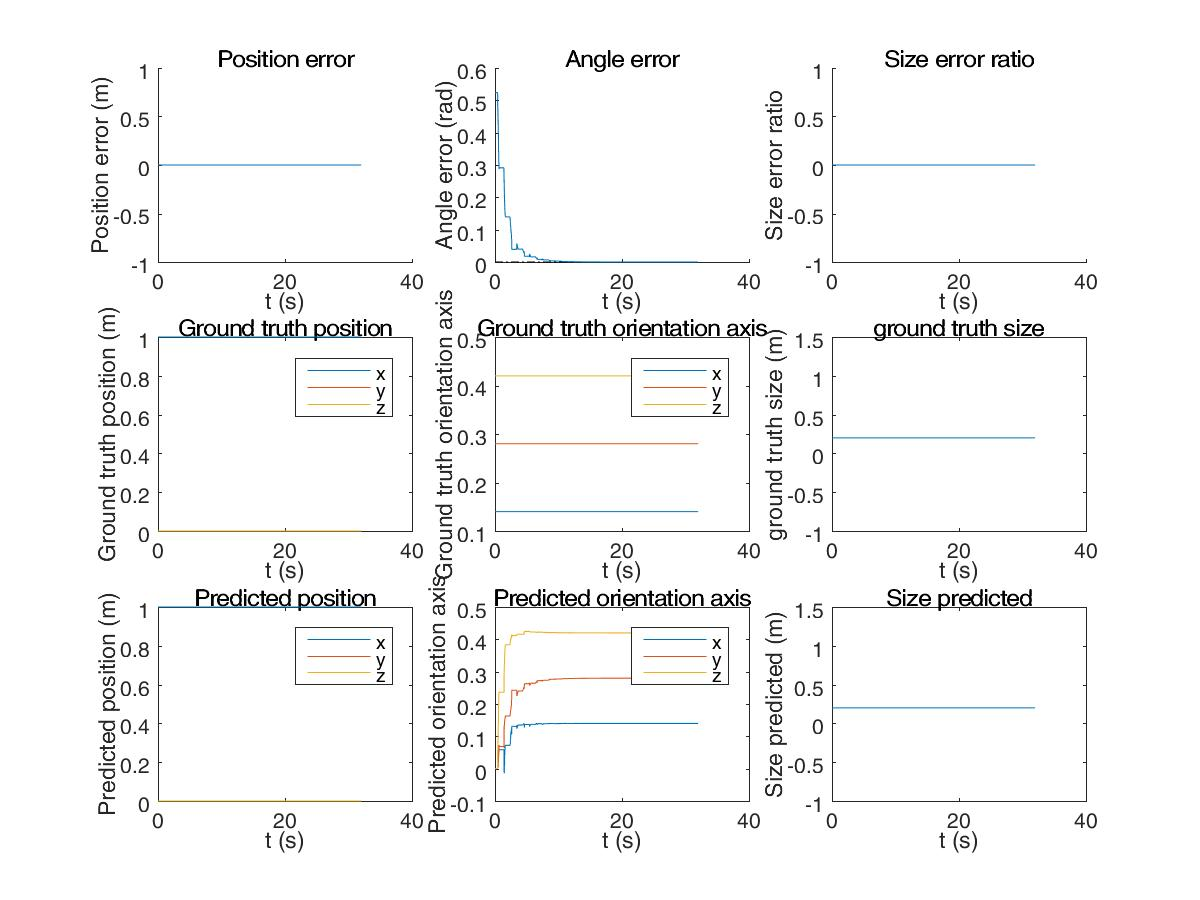
\includegraphics[width=1\textwidth,trim = 0mm 0mm 0mm 0mm,clip]{./Figures/error_xx_3F_orientation.jpg}
  \caption{Orientation correction - no noise} \label{fig:error_orientation}
\end{figure}

\begin{figure}
\centering
  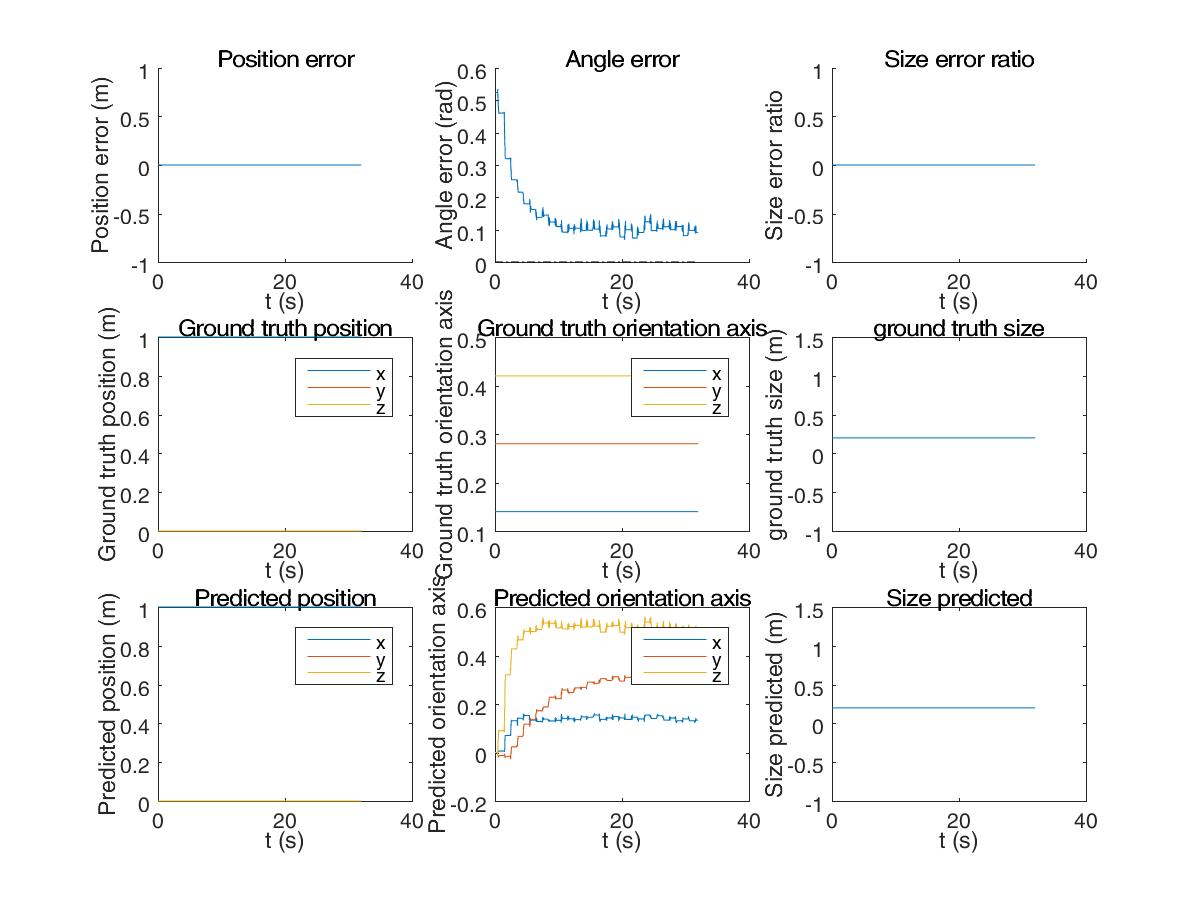
\includegraphics[width=1\textwidth,trim = 0mm 0mm 0mm 0mm,clip]{./Figures/error_xx_3F_orientation_noisy.jpg}
  \caption{Orientation correction - noise} \label{fig:error_orientation_noise}
\end{figure}

\begin{figure}
\centering
  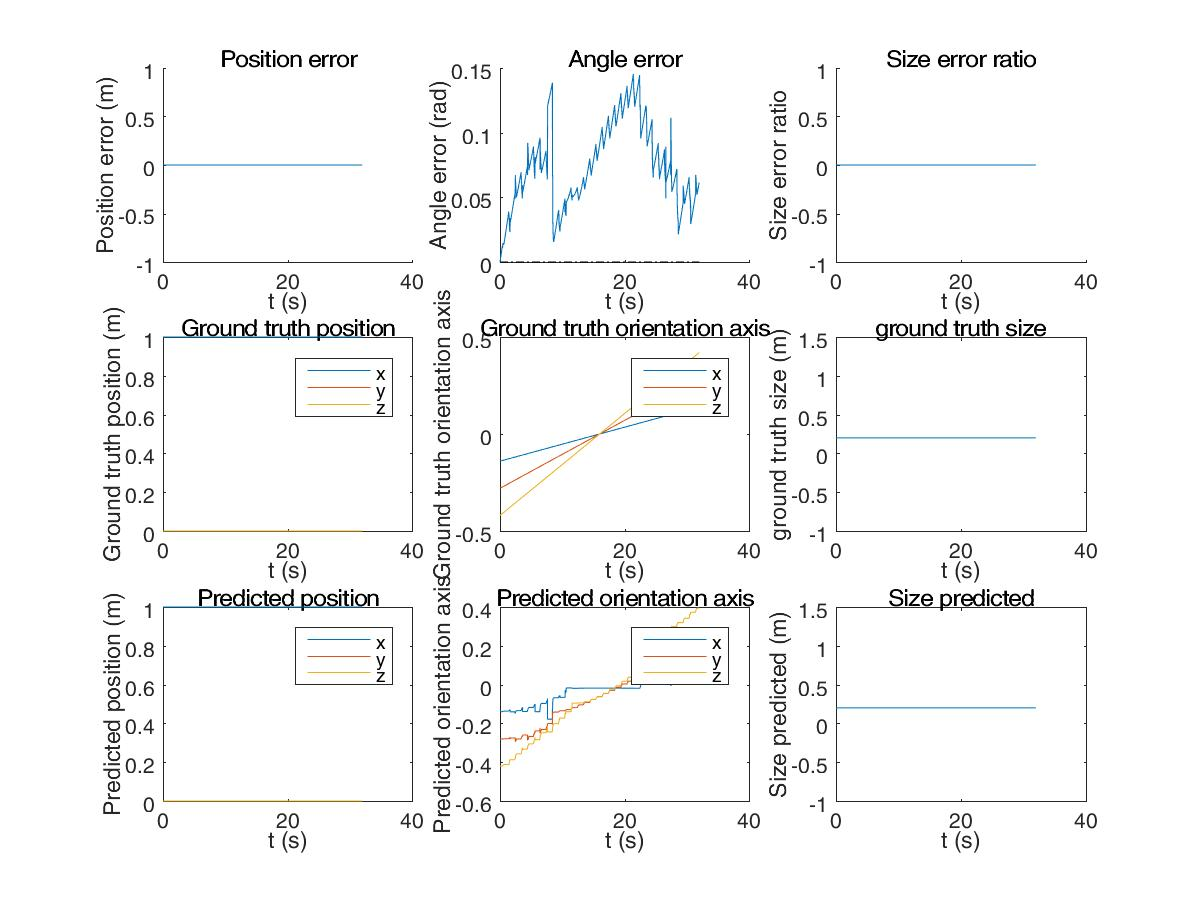
\includegraphics[width=1\textwidth,trim = 0mm 0mm 0mm 0mm,clip]{./Figures/error_Rx_3F_orientation_screw.jpg}
  \caption{rotating - Orientation correction via screw - no noise} \label{fig:error_R_orientation_screw}
\end{figure}

\begin{figure}
\centering
  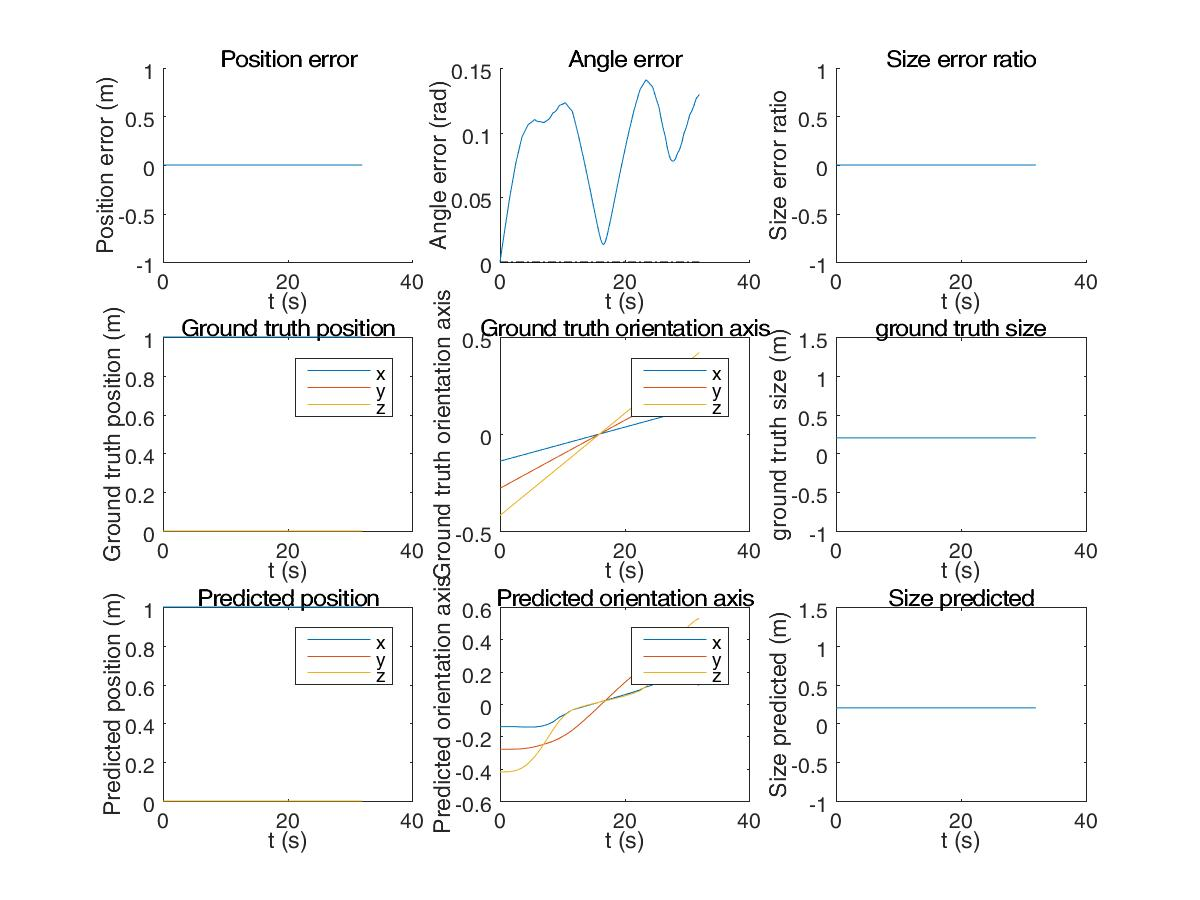
\includegraphics[width=1\textwidth,trim = 0mm 0mm 0mm 0mm,clip]{./Figures/error_Rx_3F_orientation_twist.jpg}
  \caption{rotating - Orientation correction via twist - no noise} \label{fig:error_R_orientation_twist}
\end{figure}

\begin{figure}
\centering
  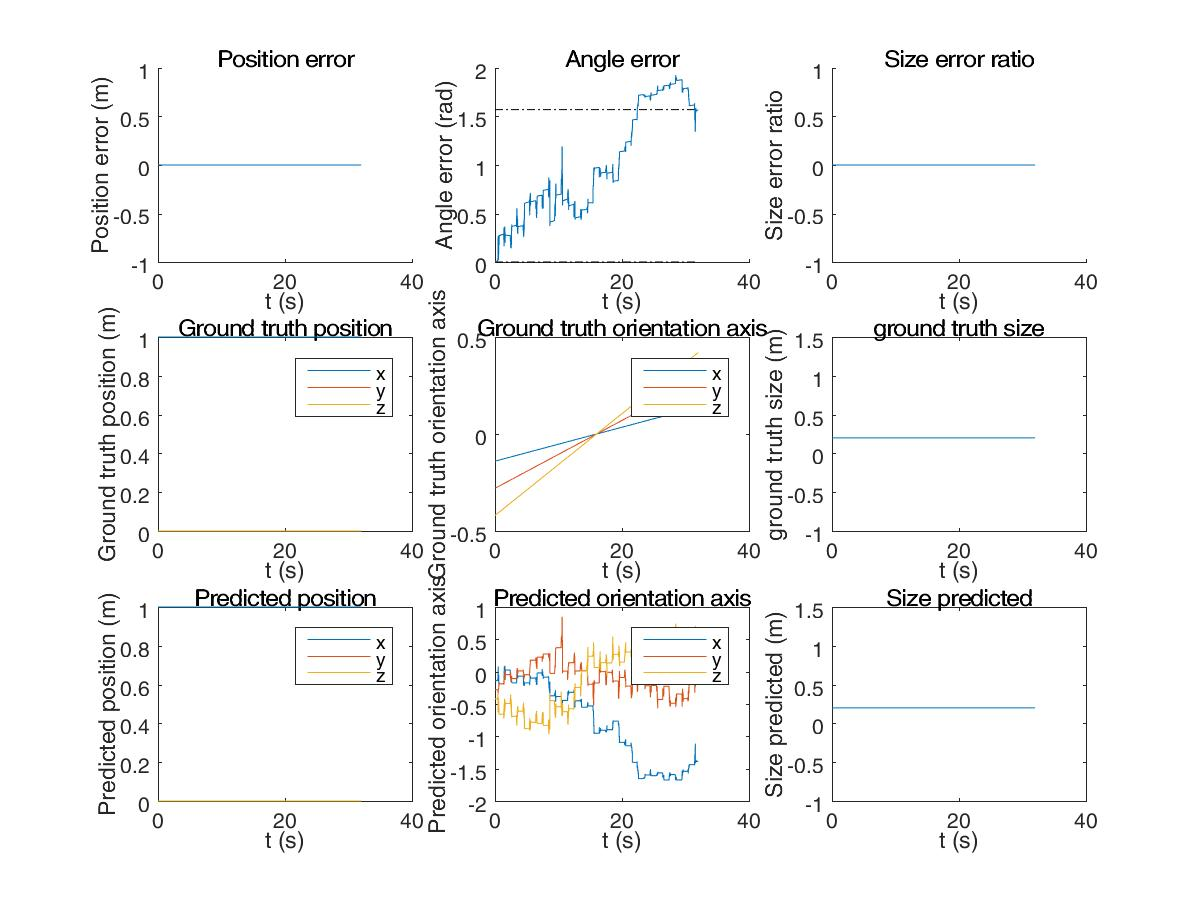
\includegraphics[width=1\textwidth,trim = 0mm 0mm 0mm 0mm,clip]{./Figures/error_Rx_3F_orientation_noise_screw.jpg}
  \caption{rotating - Orientation correction via screw - noise} \label{fig:error_R_orientation_noise_screw}
\end{figure}

\begin{figure}
\centering
  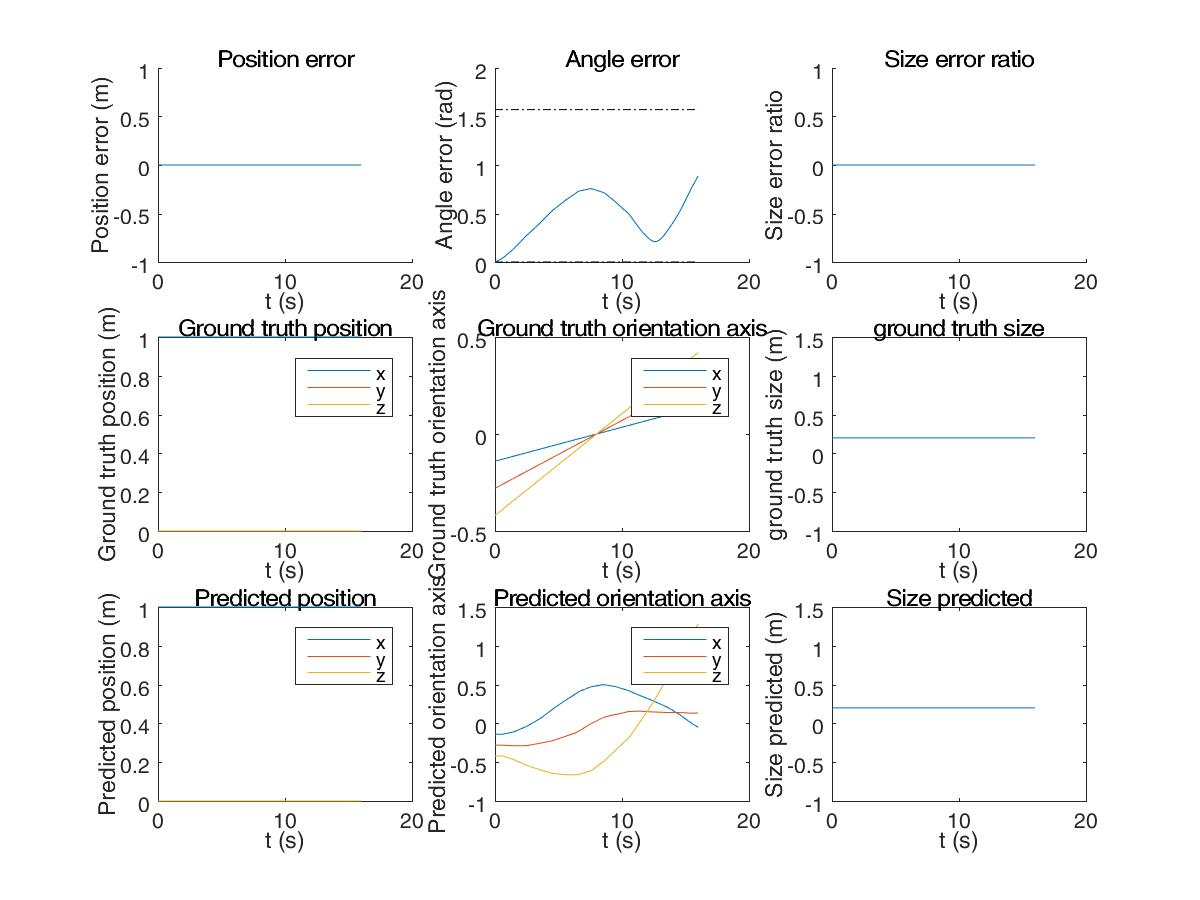
\includegraphics[width=1\textwidth,trim = 0mm 0mm 0mm 0mm,clip]{./Figures/error_Rx_3F_orientation_noise_twist.jpg}
  \caption{rotating - Orientation correction via twist - noise} \label{fig:error_R_orientation_noise_twist}
\end{figure}

\subsection{Position correction}
\textbf{PUT 3 POSITION FIGURES IN SINGLE FIGURE}
stationary - works for only 1 face visible. Without noise - Figure \ref{fig:error_1F_position}. With noise - \ref{fig:error_1F_position_noise}. 

doesnt work for 2/3 faces (results 20). Figure \ref{fig:error_2F_position}.
Requires perpendicular - multiple faces and edges mean update position vector points in wrong direction.\\

\textbf{IF THERE IS TIME, ADD TRANSLATION TRACKING}

\begin{figure}
\centering
  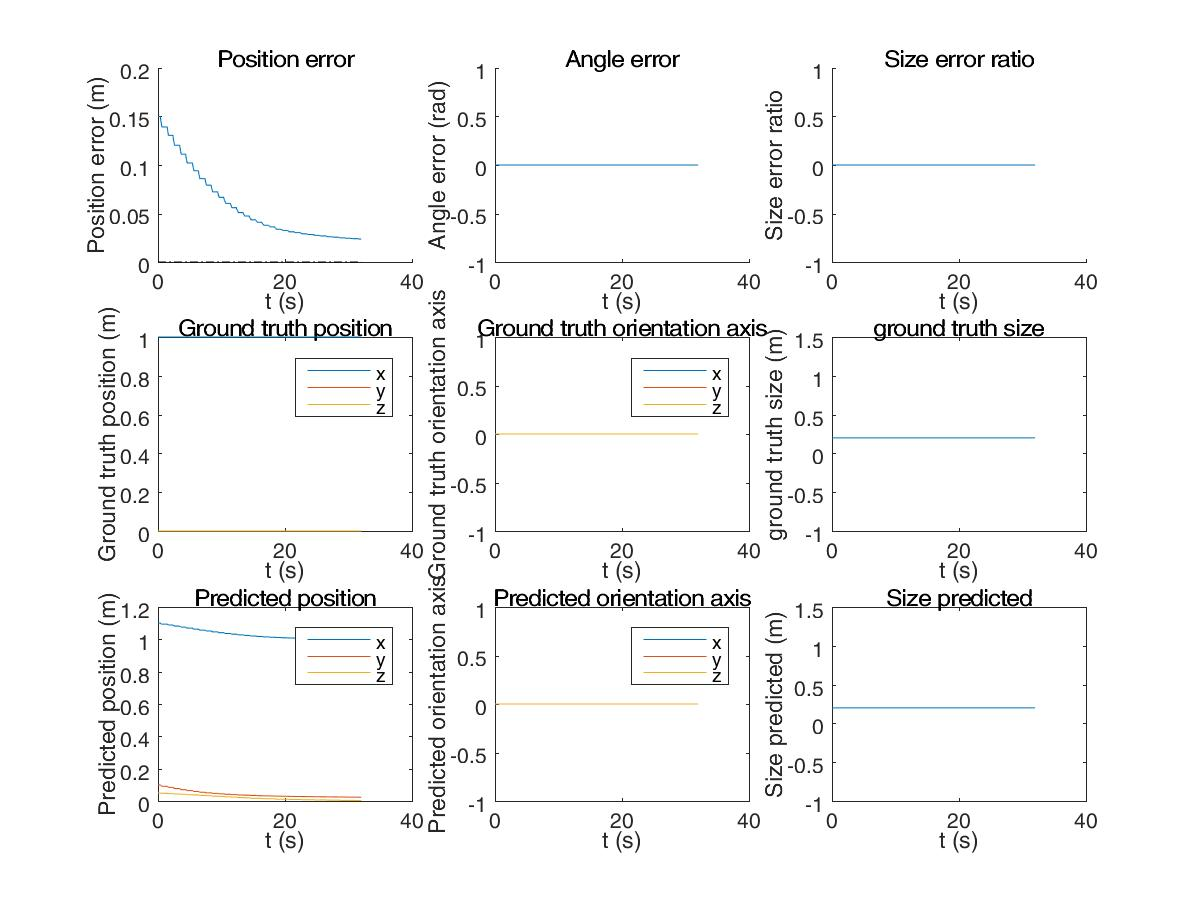
\includegraphics[width=1\textwidth,trim = 0mm 0mm 0mm 0mm,clip]{./Figures/error_1F_position.jpg}
  \caption{stationary, 1 face visible - position correction} \label{fig:error_1F_position}
\end{figure}

\begin{figure}
\centering
  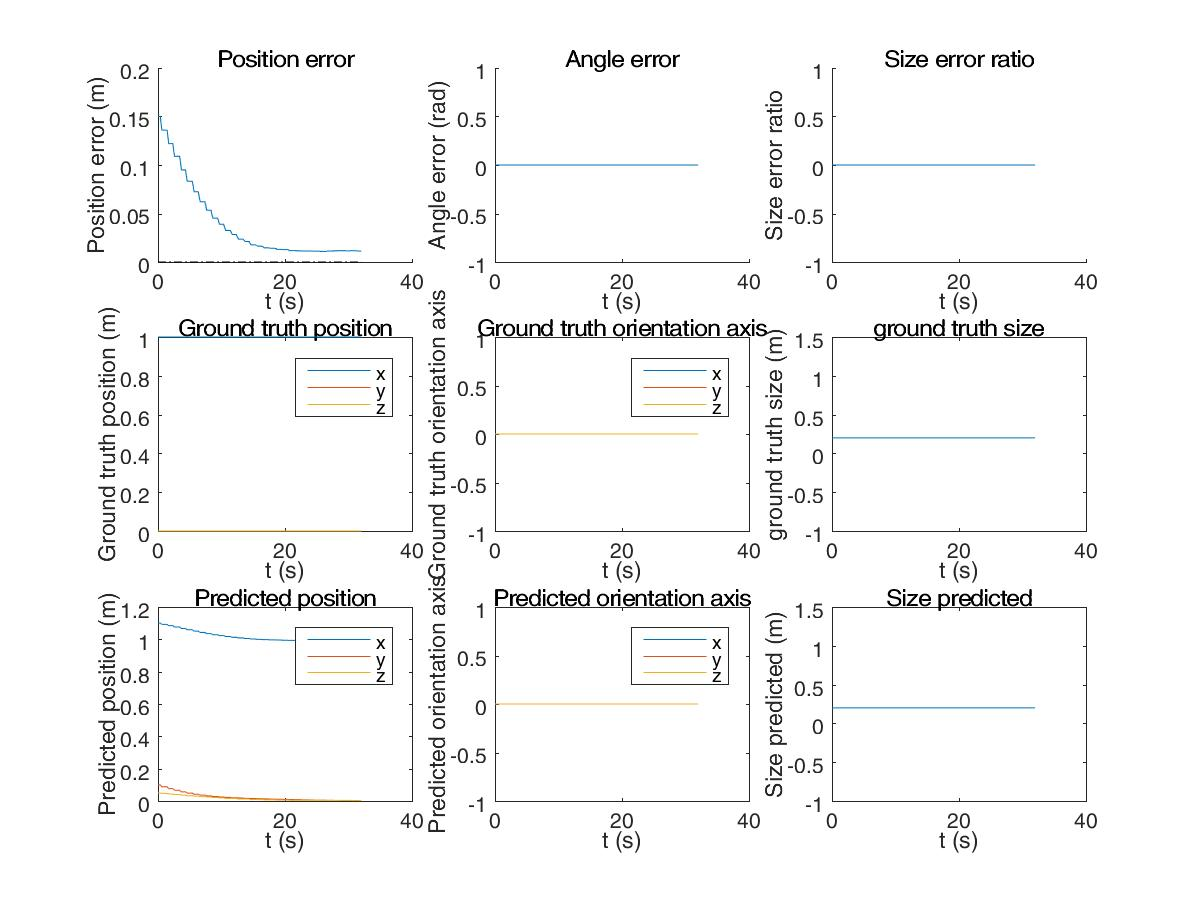
\includegraphics[width=1\textwidth,trim = 0mm 0mm 0mm 0mm,clip]{./Figures/error_1F_position_noise.jpg}
  \caption{stationary with noise, 1 face visible - position correction} \label{fig:error_1F_position_noise}
\end{figure}

\begin{figure}
\centering
  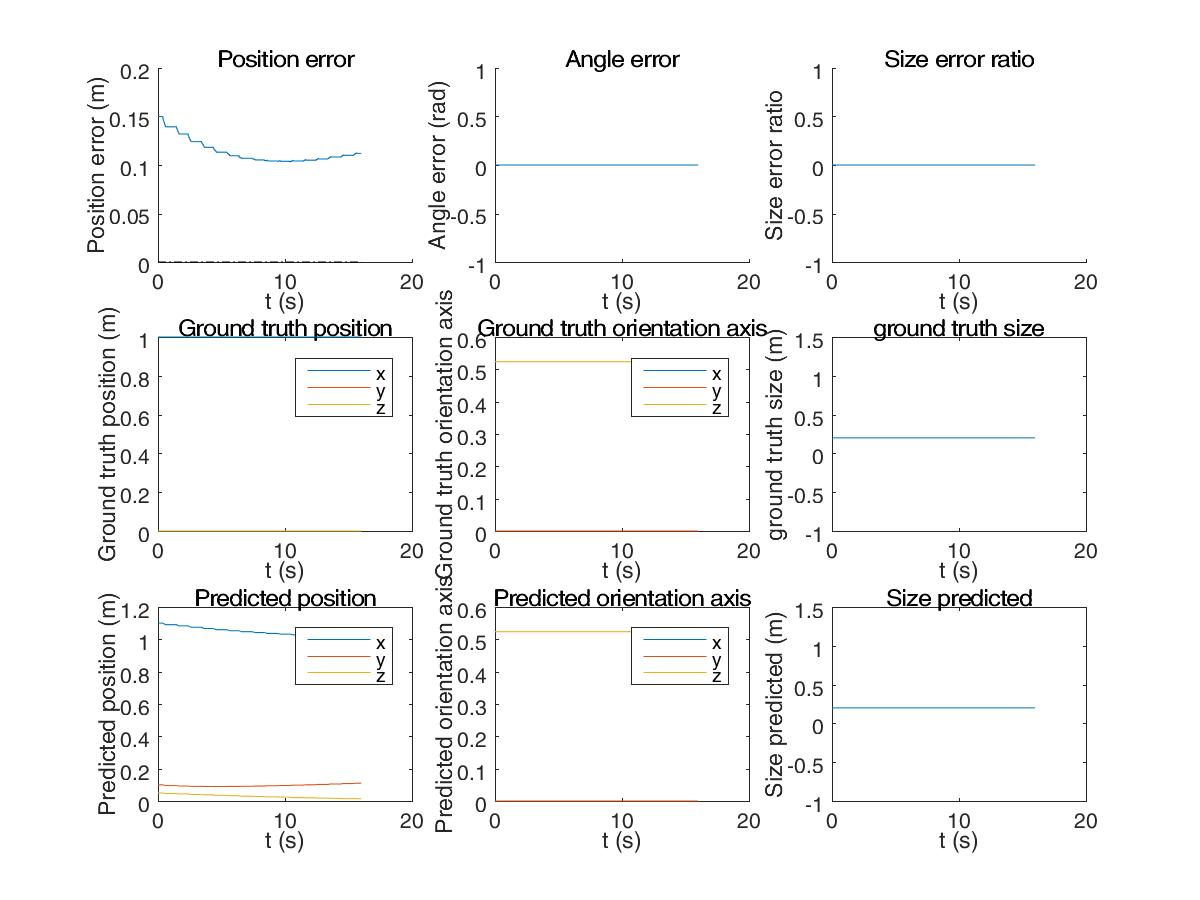
\includegraphics[width=1\textwidth,trim = 0mm 0mm 0mm 0mm,clip]{./Figures/error_2F_position.jpg}
  \caption{stationary with noise, 2 faces visible - position correction doesn't work} \label{fig:error_2F_position}
\end{figure}

\subsection{Size correction}
\textbf{PUT 2 SIZE FIGURES IN SINGLE FIGURE}
works for stationary and moving, noise and no noise, 1,2,3 faces\\
Figure \ref{fig:error_stationary_size_noise}  - noise, stationary, 3F visible - size correction\\
Figure \ref{fig:error_RT_size_noise}  - noise, rotating + translating - size correction\\

\begin{figure}
\centering
  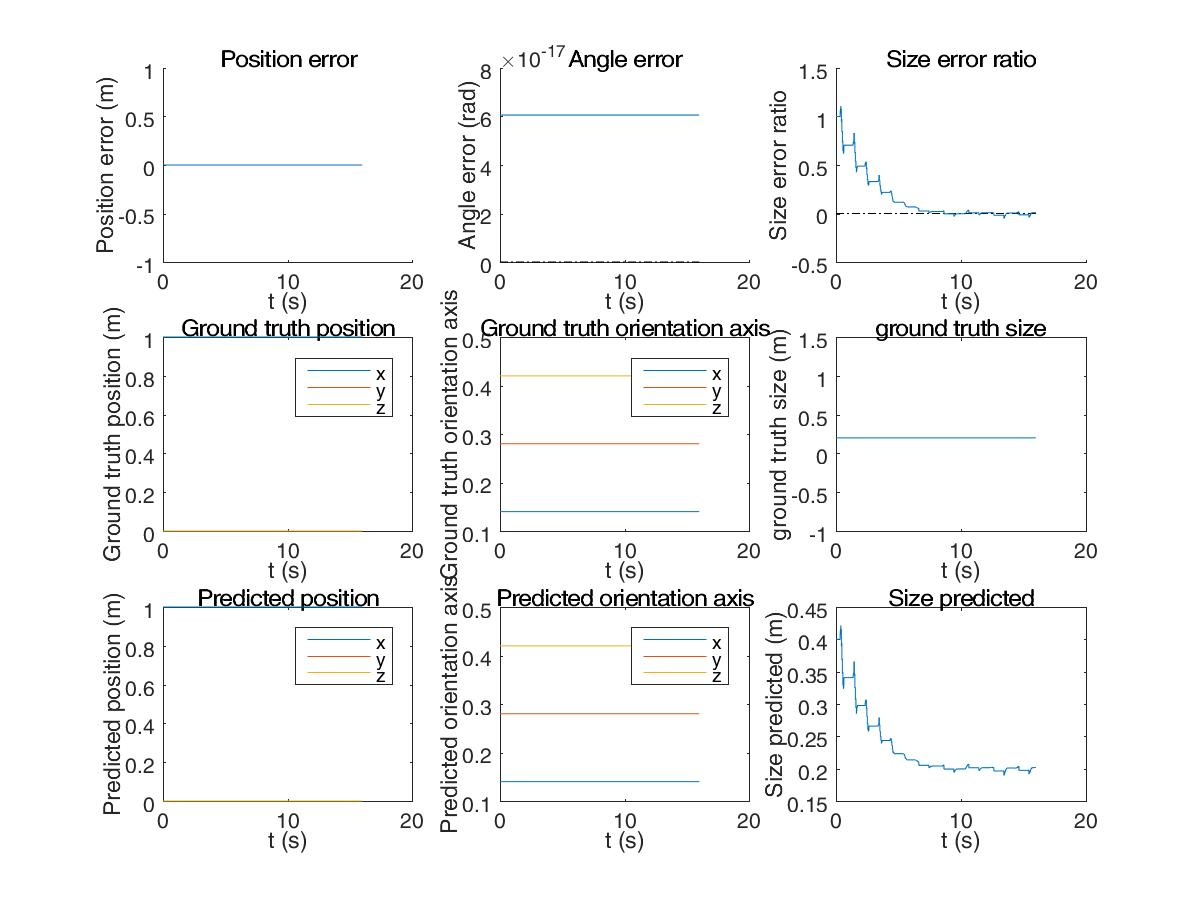
\includegraphics[width=1\textwidth,trim = 0mm 0mm 0mm 0mm,clip]{./Figures/error_xx_size_noise.jpg}
  \caption{stationary with noise, 3 faces visible - size correction} \label{fig:error_stationary_size_noise}
\end{figure}

\begin{figure}
\centering
  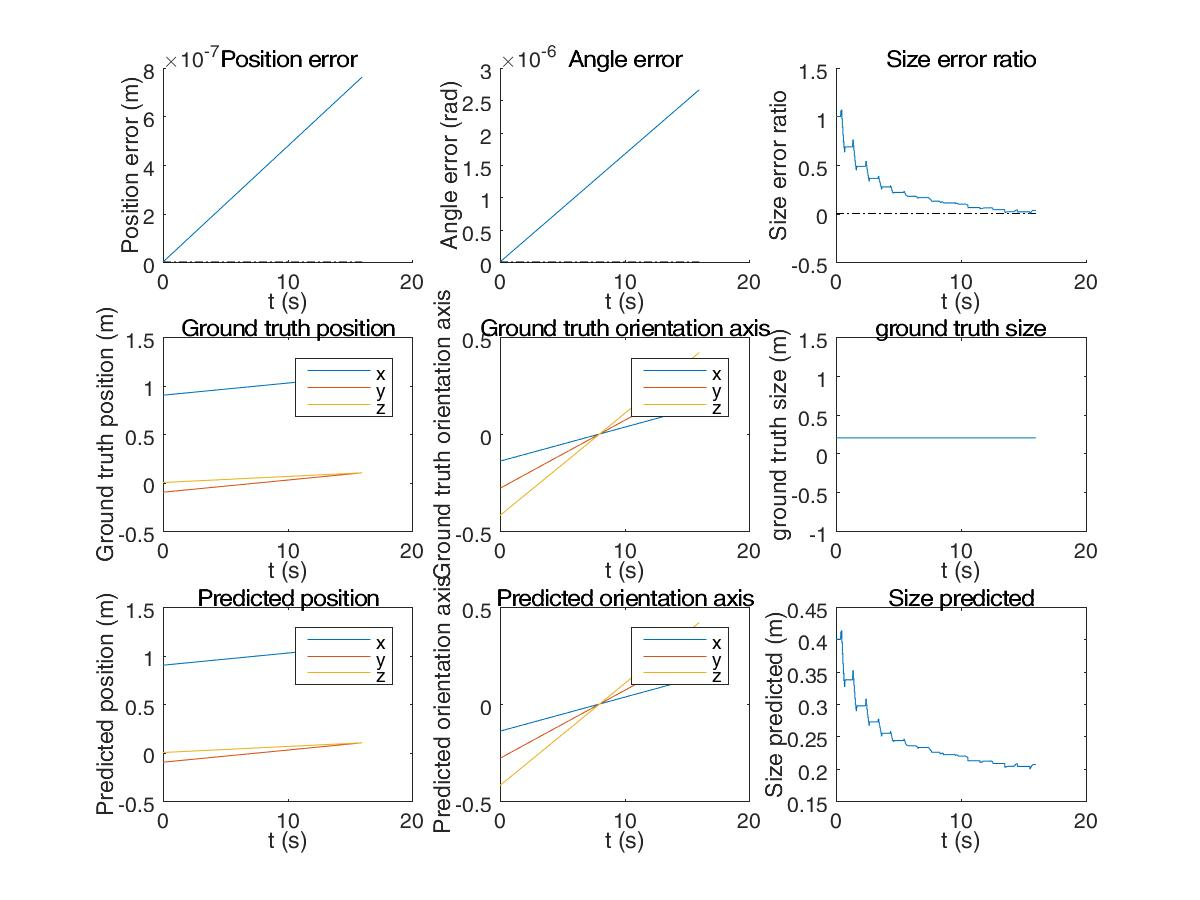
\includegraphics[width=1\textwidth,trim = 0mm 0mm 0mm 0mm,clip]{./Figures/error_RT_size_noise.jpg}
  \caption{rotating + translating with noise, 3 faces visible - size correction} \label{fig:error_RT_size_noise}
\end{figure}

\subsection{Orientation and size}
\textbf{4 separate figures. remove position plots from them; 2x3 blocks - fit 2 per page}
works in same cases orientation alone works\\
Figure \ref{fig:error_xx_3F_OxS_noise}:stationary, noisy, orientation \& size works (results 9).\\
Figure \ref{fig:error_Rx_3F_OxS_screw} - rotating, no noise, orientation updated via screw, size updated as normal. \\ 
Figure \ref{fig:error_Rx_3F_OxS_twist} - rotating, no noise, orientation updated via twist, size updated as normal.

\begin{figure}
\centering
  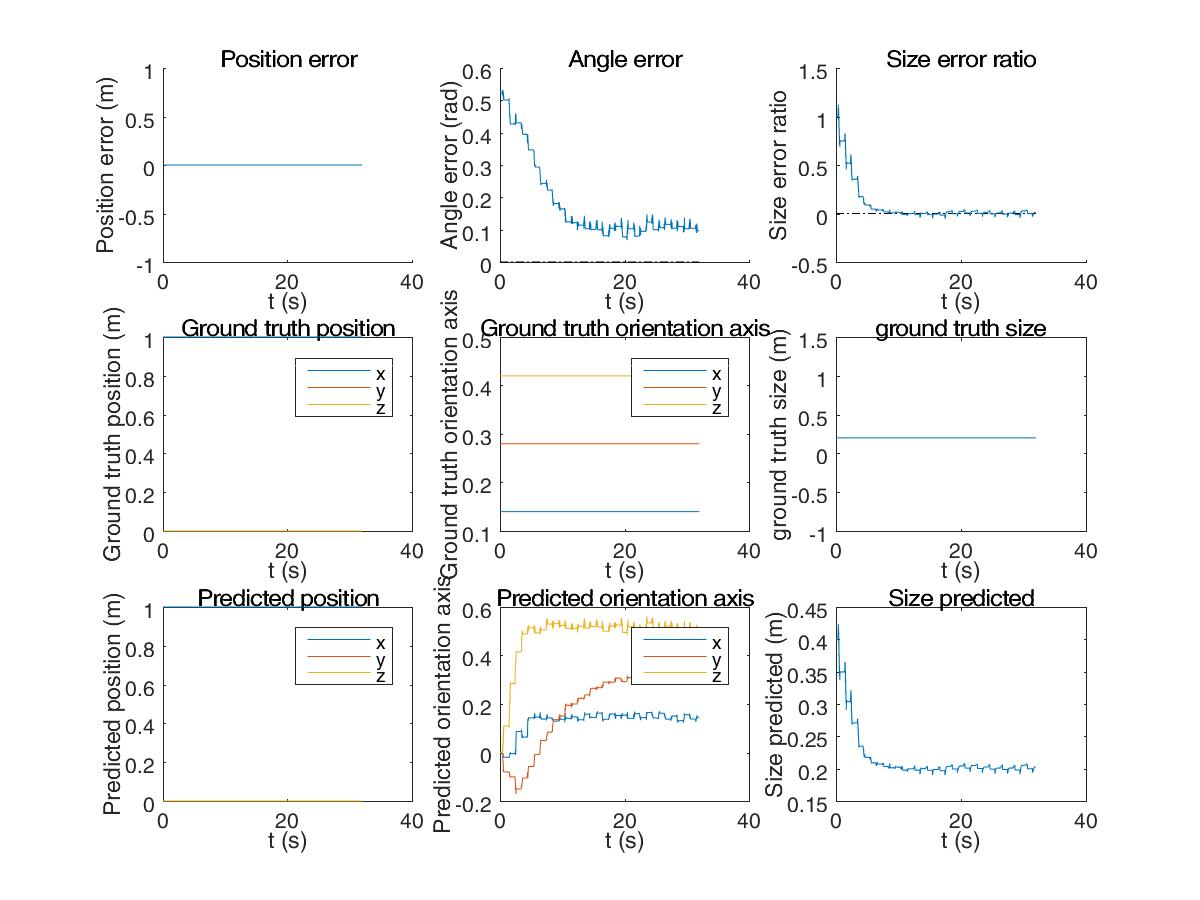
\includegraphics[width=1\textwidth,trim = 0mm 0mm 0mm 0mm,clip]{./Figures/error_xx_3F_OxS_noise.jpg}
  \caption{stationary with noise, 3 faces visible - orientation and size correction} \label{fig:error_xx_3F_OxS_noise}
\end{figure}

\begin{figure}
\centering
  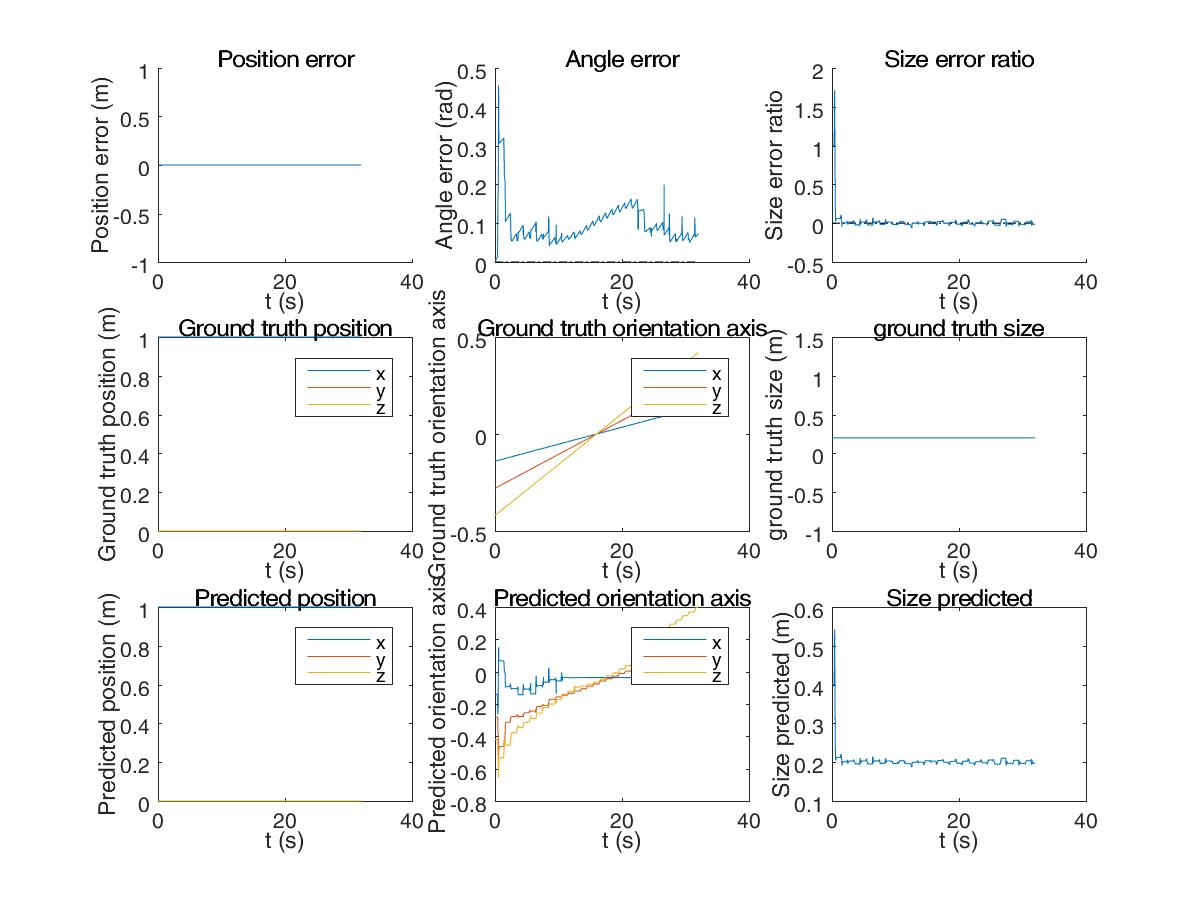
\includegraphics[width=1\textwidth,trim = 0mm 0mm 0mm 0mm,clip]{./Figures/error_Rx_3F_OxS_screw.jpg}
  \caption{rotating with no noise, 3 faces visible - orientation (via screw) and size correction} \label{fig:error_Rx_3F_OxS_screw}
\end{figure}

\begin{figure}
\centering
  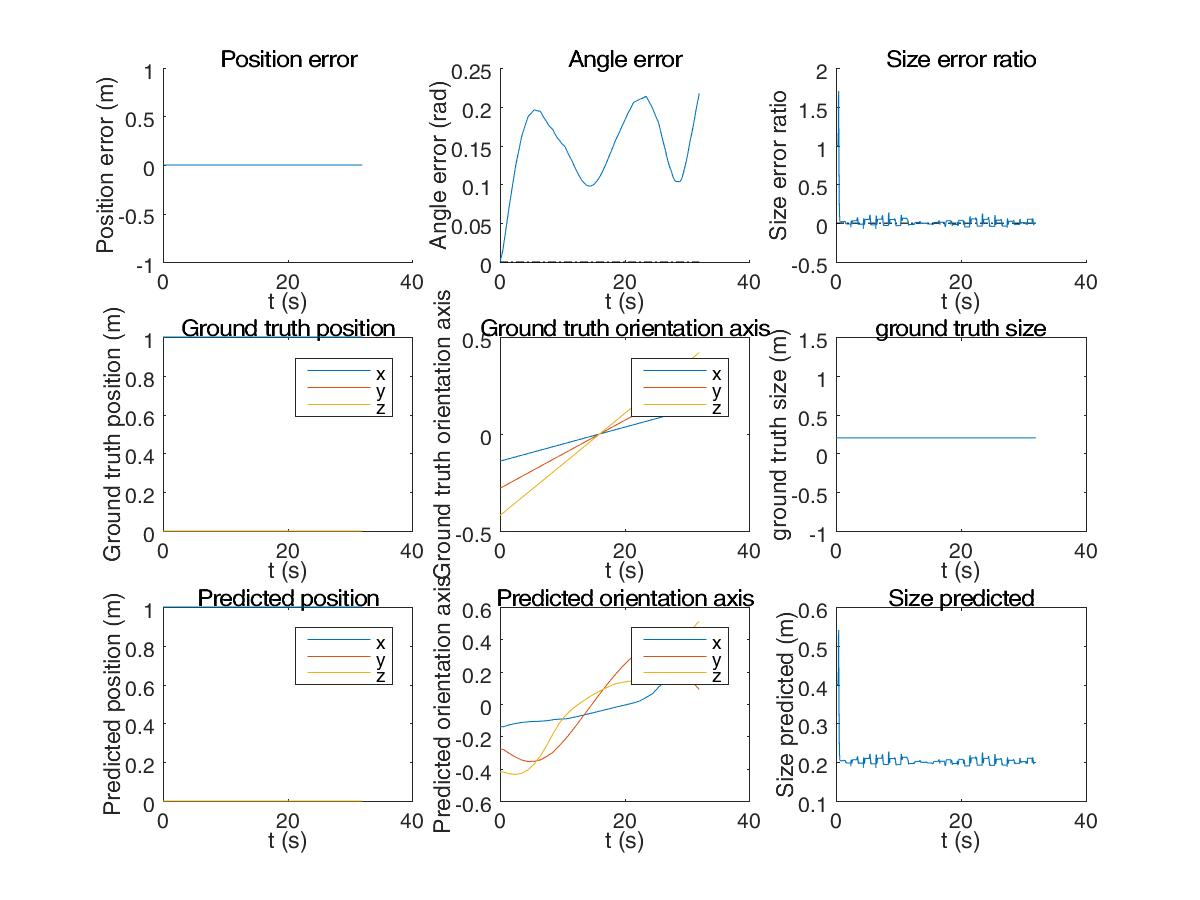
\includegraphics[width=1\textwidth,trim = 0mm 0mm 0mm 0mm,clip]{./Figures/error_Rx_3F_OxS_twist.jpg}
  \caption{rotating with no noise, 3 faces visible - orientation (via twist) and size correction} \label{fig:error_Rx_3F_OxS_twist}
\end{figure}

\subsection{discussion}
Size most robust, then orientation, then position. When combining, performance limited by less robust update.

Observer does not rely on cube shape. Replaced cube with tetrahedron, still works. Figure \ref{fig:tetrahedron}.
\begin{figure}
\centering
  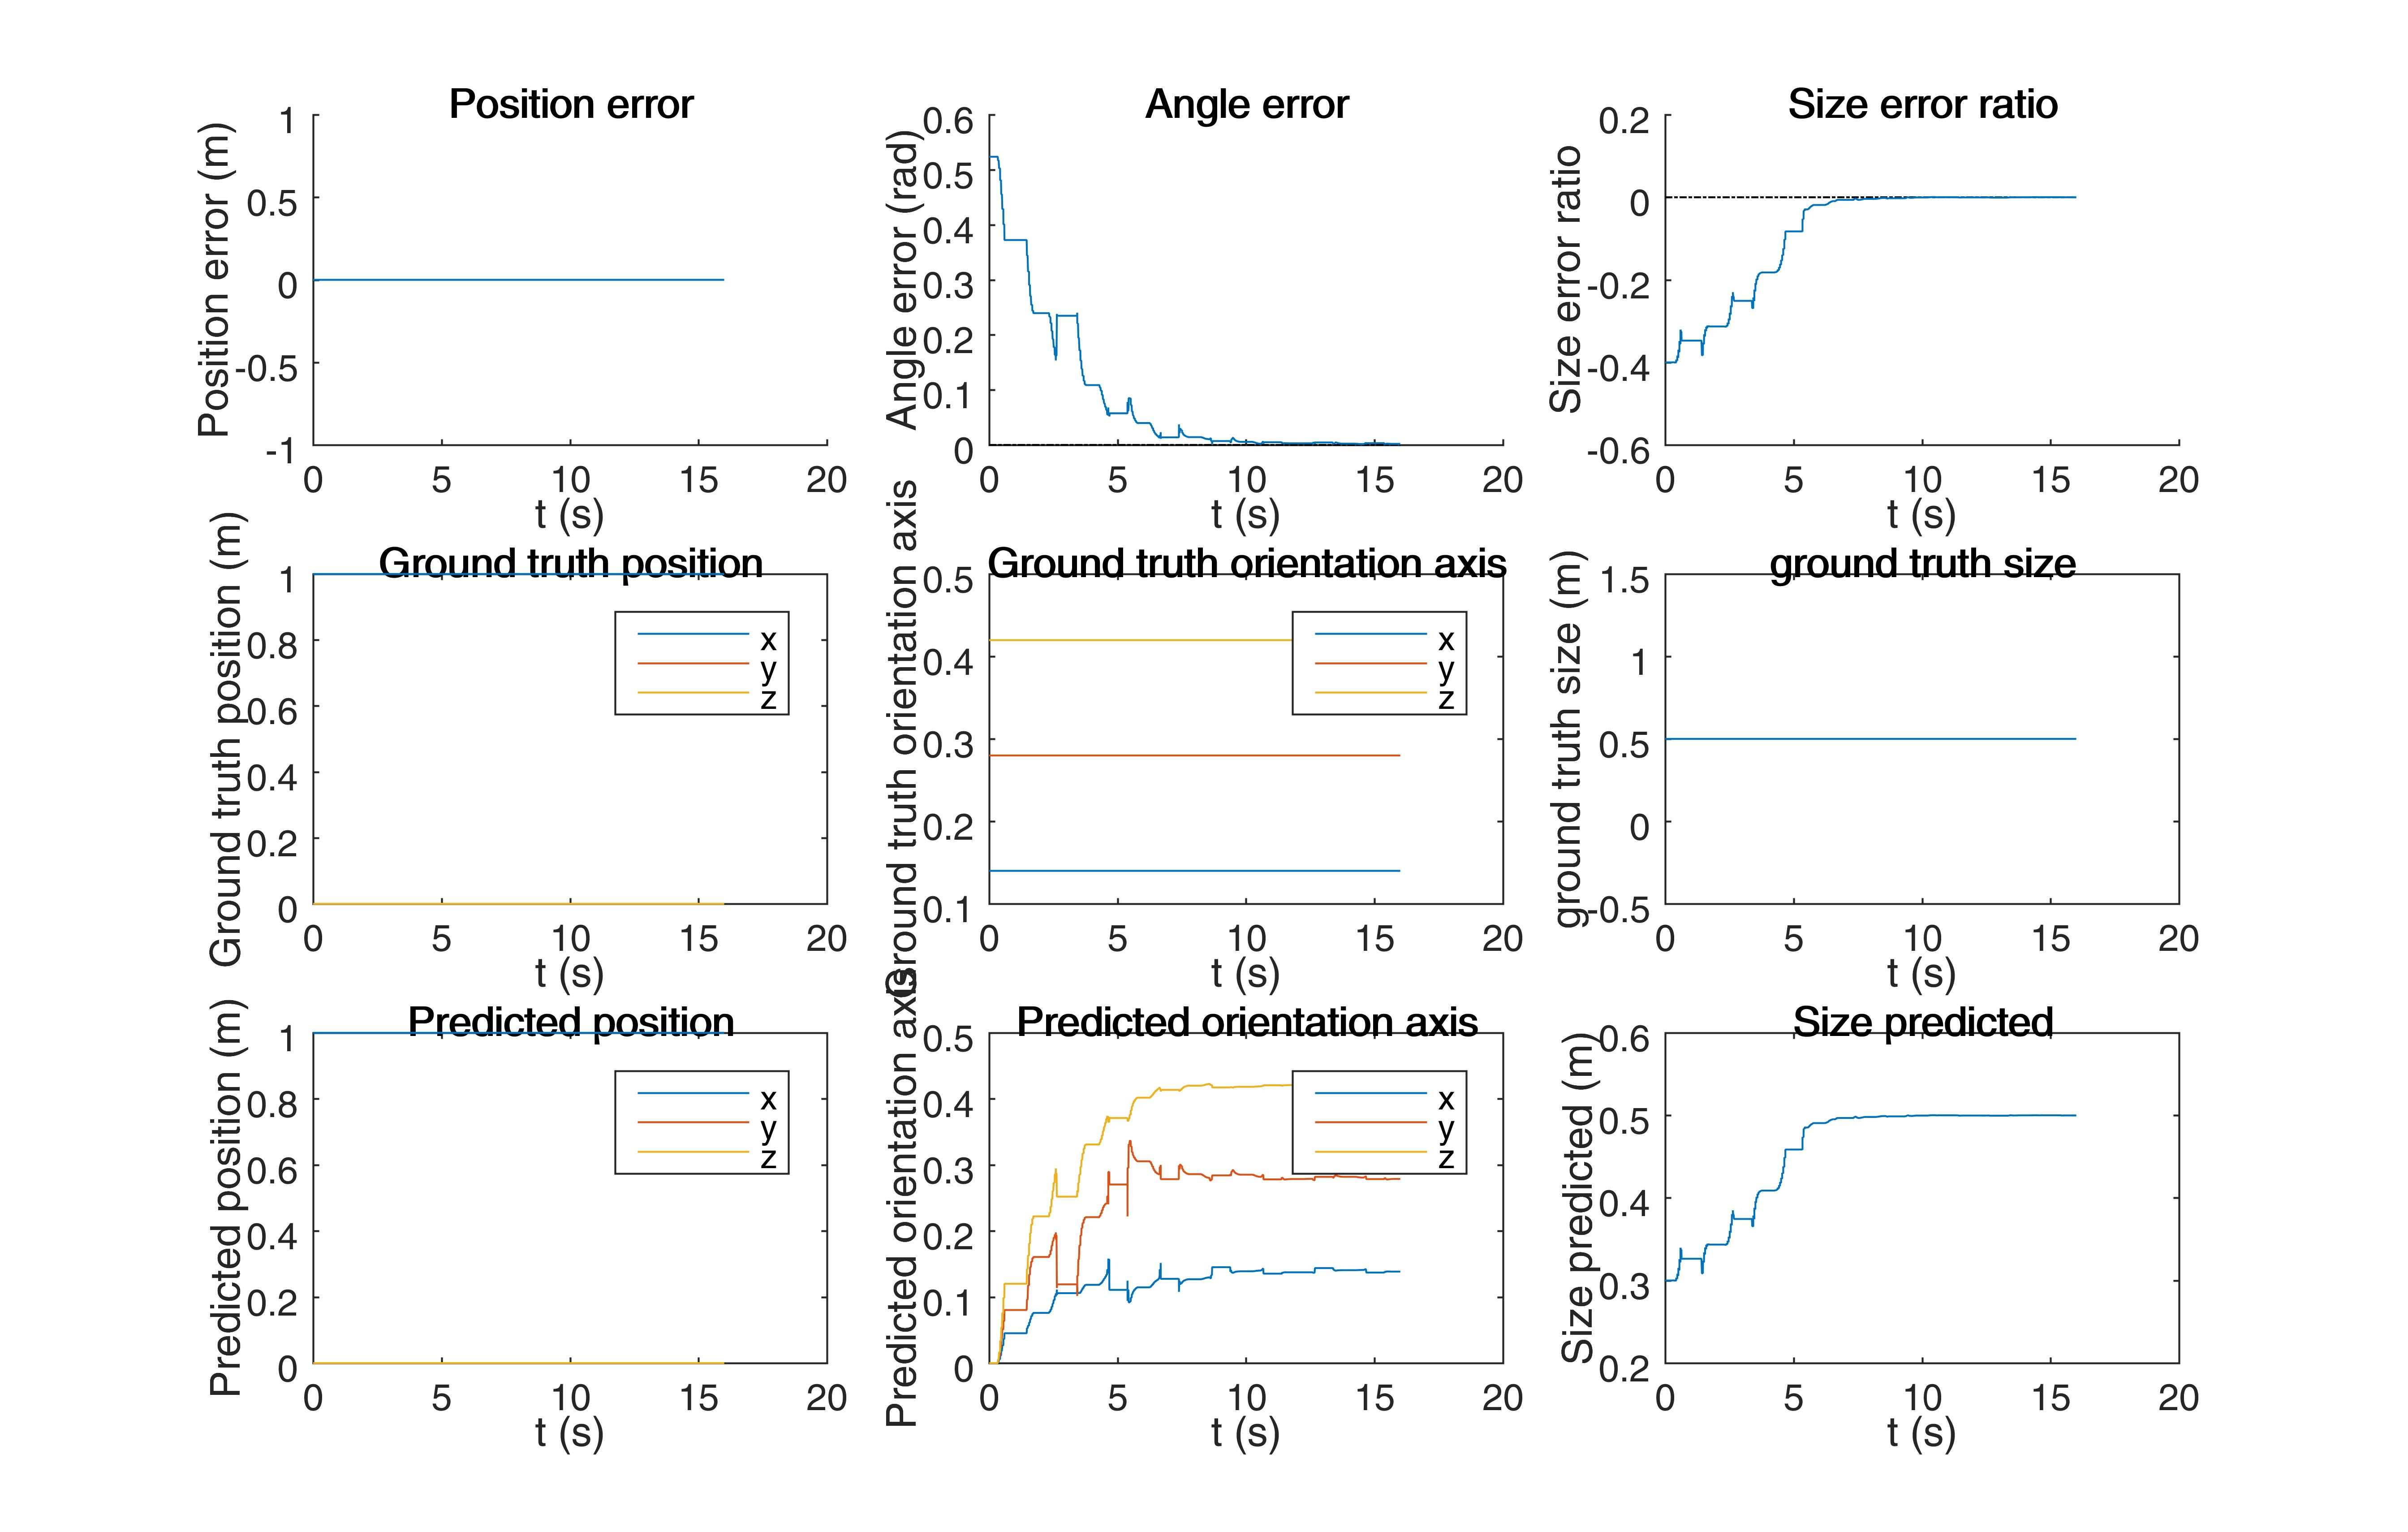
\includegraphics[width=1\textwidth,trim = 0mm 0mm 0mm 0mm,clip]{./Figures/tetrahedron_observer.jpg}
  \caption{Tetrahedron: orientation \& size correction} \label{fig:tetrahedron}
\end{figure}

Seems to be a good approach. To improve, need to fix position. Also, overshoot when adjusting via twist matrix. Twist needs very fine tuning. Instead, do some combination of screw and twist to maximise speed, minimise overshoot.
